\documentclass[11pt]{amsart}
\pdfoutput=1
\usepackage[letterpaper,margin=1in]{geometry}
\usepackage[dvipsnames]{xcolor}
\usepackage{amssymb,mathrsfs,mathtools,esint,graphicx,nicefrac,microtype}
\newcommand{\nf}{\nicefrac}
\usepackage[square]{natbib}
\AddToHook{env/thebibliography/begin}{\interlinepenalty=10000}
\usepackage[citecolor=PineGreen,colorlinks=true,linkcolor=RoyalBlue,urlcolor=BrickRed,pdfstartview=FitV]{hyperref}
\newtheorem{proposition}{Proposition}[section]
\newtheorem{theorem}[proposition]{Theorem}
\newtheorem{lemma}[proposition]{Lemma}
\newtheorem{corollary}[proposition]{Corollary}
\newtheorem{conjecture}[proposition]{Conjecture}
\theoremstyle{definition}
\newtheorem{assumption}{Assumption}[section]
\theoremstyle{remark}
\newtheorem{remark}[proposition]{Remark}
\numberwithin{equation}{section}
\newcommand{\E}{\mathbb E}
\newcommand{\Q}{\mathbb Q}
\newcommand{\R}{\mathbb R}
\newcommand{\N}{\mathbb N}
\newcommand{\Zd}{\mathbb Z^d}
\renewcommand{\a}{\mathbf a}
\renewcommand{\b}{\mathbf b}
\newcommand{\ahom}{\overline{\mathbf a}}
\newcommand{\Div}{\operatorname{Div}}
\newcommand{\cA}{\mathcal A}
\renewcommand{\epsilon}{\varepsilon}
\usepackage{tikz}
\usetikzlibrary{arrows.meta,positioning}
\newcommand{\C}{\mathbb C}
\newcommand{\dd}{\,d}
\newcommand{\diver}{\operatorname{div}}
\newcommand{\Cov}{\operatorname{Cov}}
\newcommand{\Var}{\operatorname{Var}}
\newcommand{\norm}[1]{\left\|#1\right\|}
\newcommand{\abs}[1]{\left|#1\right|}
\newcommand{\red}[1]{\textcolor{red}{#1}}
\setlength{\emergencystretch}{2em}
\title[Quantitative Einstein relation]{Quantitative Einstein relation for reversible diffusions in a random environment}
\hypersetup{pdftitle={Quantitative Einstein relation for reversible diffusions in a random environment},pdfauthor={Ahmed Bou-Rabee and Ruizhe Xu}}
\author{Ahmed Bou-Rabee}
\address{Department of Mathematics, University of Pennsylvania, Philadelphia, PA 19104}
\email{ahmedb@sas.upenn.edu}
\author{Ruizhe Xu}
\address{School of Mathematical Sciences, Zhejiang University, Hangzhou, China}
\email{ruizhexu.math@gmail.com}
\date{}
\begin{document}
\raggedbottom
\begin{abstract}
A reversible diffusion in a stationary random environment acquires a velocity under a constant force. The Einstein relation identifies the linear response with the diffusivity of the unforced particle. We prove the expansion through the first possible nonanalytic order in every dimension at least two, for smooth uniformly elliptic coefficients and a bounded potential with a finite range of dependence. The critical term is logarithmic in even dimensions and an absolute power in odd dimensions. The expansion holds for both force signs, with structurally bounded coefficients and an explicit uniform remainder. The proof identifies the correlations at the force-dependent diffusion scale by quantitative homogenization, then controls their remaining time integral by regeneration.
\end{abstract}
\maketitle
\section{Introduction}\label{sec.intro}

A particle diffusing in a disordered medium, subjected to a small constant force, eventually drifts at an asymptotic velocity. To leading order, this velocity is a linear function of the force; the proportionality matrix is called the \textbf{mobility}. The \textbf{Einstein relation} predicts that the mobility equals the diffusivity matrix of the unforced particle. We work with the formulation of~\citet*{Einstein2012gantert}: the velocity is first defined at a fixed force, and its ratio to the force magnitude is then compared with the diffusivity matrix evaluated in the force direction. We prove the full expansion through the first possible nonanalytic order, for smooth environments in every dimension $d\geq2$. The critical term is logarithmic in even dimensions and an absolute power in odd dimensions. The expansion holds for both force signs, with an explicit error bound common to laws with fixed structural data.

\begin{figure}[ht]
\centering
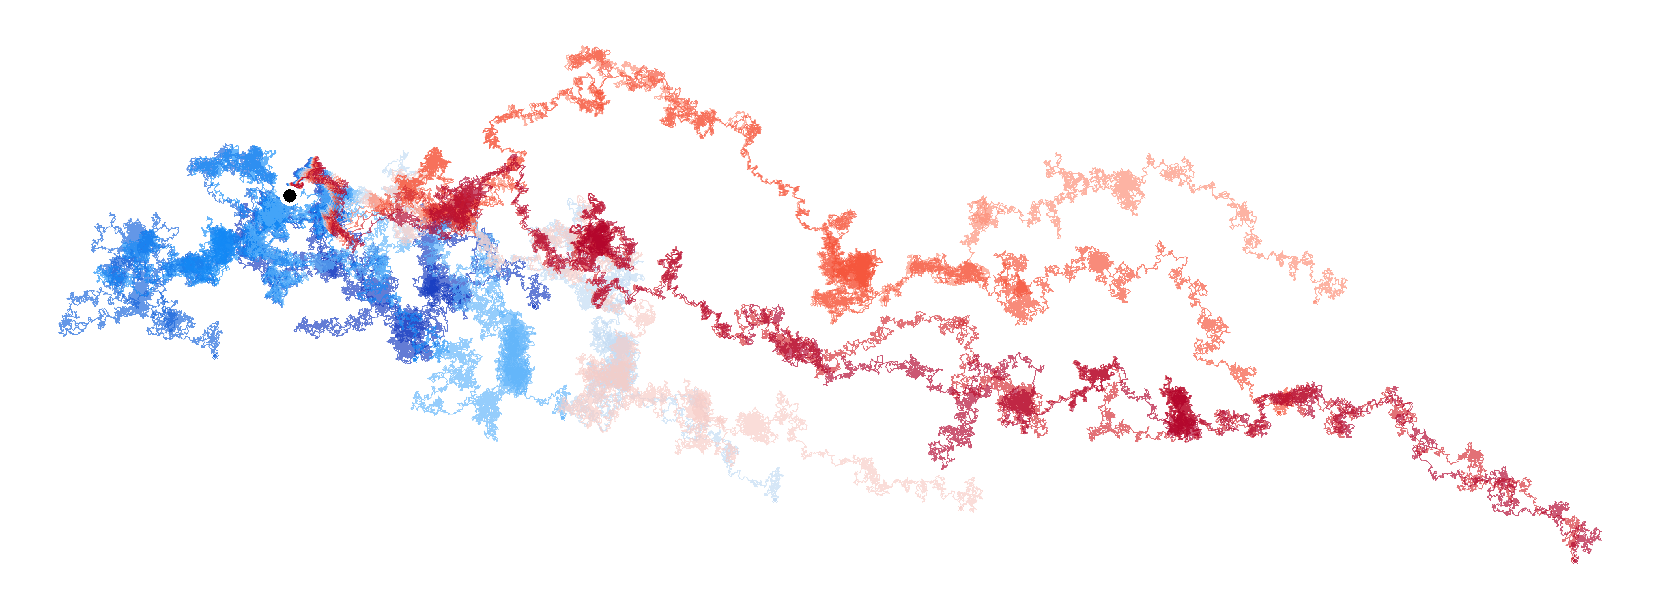
\includegraphics[width=\textwidth]{einstein_paths.pdf}
\caption{Sample paths of Brownian motions with drift~$\lambda e_1$, started from a common origin (black dot), with $\lambda$ varying continuously from $\lambda=0$ (blue) to a small positive value (red).}
\label{fig.einstein-illustration}
\end{figure}

\subsection{Setting and main results}\label{ss.setting}

Let $\a_0$ be a symmetric, uniformly elliptic random matrix field on $\R^d$, and let $V$ be a bounded random potential. The unforced particle is the reversible diffusion with generator
\begin{equation}\label{eq.physical-generator}
 \mathcal L_X^0f\coloneqq\frac12e^{2V}\nabla\cdot(e^{-2V}\a_0\nabla f)\, .
\end{equation}
Applying a signed force $\lambda\in\R$ in the direction $e_1=(1,0,\ldots,0)$ adds the drift $\lambda\a_0e_1$:
\begin{equation}\label{eq.physical-tilt}
 \mathcal L_X^\lambda f\coloneqq\mathcal L_X^0f+\lambda\a_0e_1\cdot\nabla f\, .
\end{equation}
We write $X^\lambda$ for this diffusion, started at the origin. The choice of the direction $e_1$ is without loss of generality. Precise hypotheses on the environment are as follows.

\begin{assumption}\label{a.environment}
Let $(\Omega,\mathcal F,\Q)$ be a probability space, let $\Lambda_0\geq1$, and let $r_0\geq1$. Let $(\a_0,V)$ be a measurable random field on $\R^d$ such that, almost surely,
\begin{enumerate}
\item[(S1)] $\a_0$ is symmetric and $\Lambda_0^{-1}|\xi|^2\leq\xi\cdot\a_0(x)\xi\leq\Lambda_0|\xi|^2$ for every $x,\xi\in\R^d$;
\item[(S2)] $|V(x)|\leq\Lambda_0$ for every $x\in\R^d$;
\item[(S3)] $\a_0$ and $V$ are $\Lambda_0$-Lipschitz, with matrices measured in the operator norm.
\end{enumerate}
Suppose also that the joint law of $(\a_0,V)$ satisfies
\begin{enumerate}
\item[(S4)] stationarity: it is invariant under every translation of $\R^d$;
\item[(S5)] finite range of dependence: for all Borel sets $U_1,U_2\subseteq\R^d$ with $\operatorname{dist}(U_1,U_2)>r_0$, the restrictions of $(\a_0,V)$ to $U_1$ and to $U_2$ are independent.
\end{enumerate}
\end{assumption}

For the full expansion we impose an additional smoothness hypothesis.

\begin{assumption}\label{a.smooth}
Let $(\Lambda_k)_{k\geq1}$ be positive deterministic constants. Almost surely, $\a_0,V\in C^\infty(\R^d)$ and, for every integer $k\geq1$,
\begin{equation}\label{e:smooth-hypothesis}
 \|\nabla^k\a_0\|_\infty+\|\nabla^kV\|_\infty\leq\Lambda_k\, .
\end{equation}
\end{assumption}

Write $\mathcal D=(d,\Lambda_0,r_0,(\Lambda_k)_{k\geq1})$ for the \textbf{structural data}. A structural constant is common to this class of laws; each estimate below uses only finitely many derivative bounds.

Under Assumption~\ref{a.environment}, the unforced diffusion satisfies the invariance principle of~\citet*{DeMasiFerrariGoldsteinWick1989}: as $\epsilon\downarrow0$, the process $\epsilon X^0(\epsilon^{-2}t)$ converges in law to Brownian motion with covariance $t\Sigma_X$, for a deterministic effective diffusivity $\Sigma_X$. For fixed $\lambda\neq0$, the diffusion has a deterministic velocity:
\begin{equation}\label{eq.velocity-definition}
 \lim_{t\to\infty}\frac{X^\lambda(t)}t=\ell_X(\lambda)
 \quad\text{almost surely, for almost every environment}\, .
\end{equation}
This law of large numbers follows from the regeneration times of~\citet*{ballistic2003shen,ballistic2004shen}, in the force-dependent form constructed by~\citet[Section~5]{Einstein2012gantert}. For negative force the construction is applied in direction $-e_1$. Set $\ell_X(0)=0$.

Our result retains every ordinary coefficient through degree $d+1$, together with the critical term. Define, for $0<s\leq e^{-1}$,
\begin{equation*}
 \omega(s)\coloneqq\exp\bigl(-\sqrt{\log(1/s)}\bigr),\qquad
 T_d(\lambda)\coloneqq\begin{cases}
 \lambda^d\log(1/|\lambda|),&d\text{ even},\\
 |\lambda|^d,&d\text{ odd},
 \end{cases}\, ,
\end{equation*}
and set $S_d(\lambda)\coloneqq\lambda T_d(\lambda)$.

\begin{theorem}\label{t:expansion}
For every $d\geq2$ and structural data set $\mathcal D$, there exist $C(\mathcal D)<\infty$ and $\lambda_*(\mathcal D)\in(0,e^{-1}]$ such that every law satisfying Assumptions~\ref{a.environment} and~\ref{a.smooth} has deterministic vectors $b_1,\ldots,b_{d+1},c\in\R^d$ with
\begin{equation}\label{e:coefficient-bounds}
 b_1=\Sigma_Xe_1,\qquad \sum_{j=1}^{d+1}|b_j|+|c|\leq C\, ,
\end{equation}
and, for every real $\lambda$ with $0<|\lambda|\leq\lambda_*$,
\begin{equation}\label{e:expansion}
 \left|\ell_X(\lambda)-\sum_{j=1}^{d+1}b_j\lambda^j-cS_d(\lambda)\right|
 \leq C|\lambda|^{d+1}\omega(|\lambda|)\, .
\end{equation}
\end{theorem}

The constants and the force threshold are chosen before the environment law. The conclusion includes the finite coefficient $b_{d+1}$ even when a logarithmic term occurs at the same degree. In particular, it gives the quantitative Einstein relation as a first-order consequence.

\begin{theorem}\label{t.main}
Let $d\geq2$, and let $(\a_0,V)$ satisfy Assumptions~\ref{a.environment} and~\ref{a.smooth}. There exist $C(\mathcal D)<\infty$ and $\lambda_*(\mathcal D)>0$ such that, for every $0<\lambda\leq\lambda_*$,
\begin{equation}\label{eq.main-rate}
 \left|\frac{\ell_X(\lambda)}\lambda-\Sigma_Xe_1\right|
 \leq C\lambda\, .
\end{equation}
\end{theorem}

The same estimate holds with $|\lambda|$ for negative force. The first version~\citep{BouRabeeXu2026v1} proved a quenched power-rate estimate under Lipschitz hypotheses. The order is optimal: Proposition~\ref{sharp.example} gives smooth environments for which the mobility error has a nonzero linear term. In that construction, the time-changed velocity has first component exactly $\lambda$, and the quadratic term in the original velocity comes from the clock.

\subsection{Proof strategy}\label{ss.strategy}

The starting point is a balance of scales. Under a force of magnitude $|\lambda|$, the displacement $|\lambda|t$ caused by the force and the diffusive fluctuation $\sqrt t$ are comparable when $t\asymp|\lambda|^{-2}$, on spatial scales of order $|\lambda|^{-1}$. A time change moves the potential into the coefficient field $\a=e^{-2V}\a_0$, and leaves $\mu=e^{-2V}$ in the clock. Exact response expresses the velocity and clock through time correlations of local fields (Section~\ref{sec.notation}). At time $t$, both fields in each correlation become homogeneous drift--diffusion averages of the stationary homogenization commutator or the centered clock. Their joint covariance has a white-noise limit with a power rate. Gaussian convolution gives a profile $t^{-1-\nf d2}(u_0+u_2z^2)e^{-\gamma z^2}$ with $z=\lambda\sqrt t$. Its Taylor terms give ordinary powers; its critical Mellin integral gives a logarithm in even dimension and $|\lambda|^d$ in odd dimension. Response adds one force factor. The correlation after subtraction of this profile retains the finite coefficient at the critical degree, and division by the clock adds the commutator--clock cross covariance.

First, we control the correlation tail by regeneration (Section~\ref{regen.sec}). The environmental factorization proved in Appendix~\ref{app:regeneration}, based on~\citet[Proposition~5.4]{Einstein2012gantert}, separates the environment before a selected bridge from the environment ahead of it. A uniform renewal estimate then gives exponential decay for correlations of functions whose supports grow on the scale $|\lambda|^{-1}$. Applying this estimate after both fields have evolved for time $|\lambda|^{-2}$ preserves their small norms.

Second, we estimate the forced semigroup and its weak flux (Sections~\ref{sec.entropy} and~\ref{sec.correctors}). We adapt the spatial-average iteration in the proof of~\citet*[Theorem~9.1]{AKM2019book}. The unforced scalar and flux correctors give an exact identity for the weak flux of the actual forced solution. Locality permits conditioning its blocks on separated environments; independence then retains the central-limit factor. The resulting losses are summable over dyadic scales. The same argument applies to complex force on a fixed scaled disc. The additive structure of~\citet[Theorem~4.6]{AKM2019book} gives the joint covariance of the commutator and clock, again by independent localized blocks.

Finally, we split the evolution at a late intermediate time (Section~\ref{sec.rate}). We first replace the force in the early part of the evolution and identify the finite-time flux with the unforced commutator. Homogeneous propagation gives the Gaussian profile on a fixed complex disc and a growing real window. The complex disc controls its Taylor coefficients; the real window reaches the time at which the regeneration tail applies. Integrating and dividing by the clock gives Theorem~\ref{t:expansion}. Only first correctors and second moments of the fluctuation limit enter.

\begin{center}
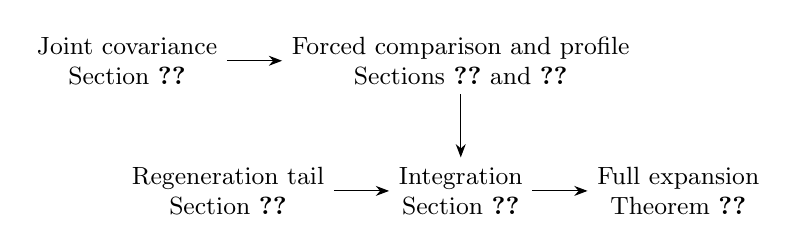
\begin{tikzpicture}[node distance=8mm and 7mm, every node/.style={align=center,font=\small},>=Stealth]
\node (static) {Joint covariance\\Section~\ref{s:covariance}};
\node[right=of static] (profile) {Forced comparison and profile\\Sections~\ref{s:gauge} and~\ref{sec.rate}};
\node[below=of profile] (integral) {Integration\\Section~\ref{s:integration}};
\node[left=of integral] (tail) {Regeneration tail\\Section~\ref{s:response}};
\node[right=of integral] (result) {Full expansion\\Theorem~\ref{t:expansion}};
\draw[->] (static)--(profile);
\draw[->] (profile)--(integral);
\draw[->] (tail)--(integral);
\draw[->] (integral)--(result);
\end{tikzpicture}
\end{center}

\subsection{Higher-order response}\label{ss.intro-sharpness}

The expansion distinguishes an ordinary power from a term with different coefficients on the two sides of zero. In dimension two, it gives
\begin{equation*}
 \frac{\ell_X(\lambda)}\lambda
 =\Sigma_Xe_1+b_2\lambda+c\lambda^2\log(1/|\lambda|)
 +b_3\lambda^2+O\bigl(|\lambda|^2\omega(|\lambda|)\bigr)\, .
\end{equation*}
In odd dimensions, the critical term $c\lambda|\lambda|^d$ is an ordinary power on each half-line, with opposite coefficients. If $c\neq0$, then it prevents a two-sided Taylor expansion through degree $d+1$. The ordinary coefficients retain the short-time correlations, whereas the critical coefficient is determined by the effective diffusivity and the joint covariance of the commutator and clock.

Perturbative calculations in the physics literature predicted these dimension-dependent terms. In dimension two,~\citet*{LeitmannFranosch2013} found a cubic logarithmic velocity term for a driven lattice Lorentz gas, to first order in obstacle density.~\citet{Novikov2018} obtained a logarithmic mobility correction by expansion in the strength of a Gaussian random potential. In dimension three,~\citet*{LeitmannBenichouFranosch2018} found a velocity term proportional to $\lambda|\lambda|^3$, again to first order in obstacle density; this term also appeared in the dilute colloidal calculation of~\citet*{SquiresBrady2005}. The obstacle models are not uniformly elliptic, and the Gaussian potential is unbounded. Theorem~\ref{t:expansion} proves the same forms in the smooth uniformly elliptic class without a small-disorder assumption.

If the joint law is also invariant under $x\mapsto-x$, then $\ell_X(-\lambda)=-\ell_X(\lambda)$, so the even polynomial coefficients vanish. The mobility error is then at most $C\lambda^2\log(1/|\lambda|)$ in dimension two and $C\lambda^2$ in higher dimensions.

Open questions include removal of the smoothness assumption, the possible signs of $c\cdot e_1$, and conditions forcing $c=0$. One may also ask whether the expansion continues to every order in integer powers and logarithms.

\subsection{Background}\label{ss.background}

The Einstein relation is a prototype of fluctuation--dissipation: the principle that the equilibrium fluctuations of a system determine its response to a small external perturbation. Here the fluctuation is the diffusive spreading of the unforced particle, described by the invariance principle, and the response is the velocity induced by the force. Fluctuation--dissipation and reciprocity principles were developed by \citet{Nyquist1928,Onsager1931,Onsager1931II,CallenWelton1951}; a rigorous Markov-process formulation appears in \citet{DemboDeuschel2010}.

For a test particle in a stationary random environment, the Einstein relation has been approached in three ways, which differ in how the small-force and long-time limits are ordered. \citet{LebowitzRost1994} coupled the two limits, scaling the force together with a diffusive rescaling of space and time. The remaining two approaches both send time to infinity at a fixed force, but extract different objects from that limit. \citet{Steady2018mathieu} and \citet*{GantertGuoNagel2017} studied an invariant measure, the steady state, for the environment seen from the biased particle, and recovered the Einstein relation from the small-force expansion of that measure. In our continuous reversible setting, \citet{Steady2018mathieu} constructed the steady state, proved continuity and differentiability estimates for its action on local divergences, and identified its derivative at zero force through the unforced corrector. On $\Zd$ in dimensions $d\geq3$, \citet*{GantertGuoNagel2017} obtained the analogous first-order expansion for the random conductance model, building on the variance-decay estimates of \citet{vardecay} and \citet{deBuyerMourrat2015}. Early constructions of steady states in related settings are due to \citet{KomorowskiKrupa2004}, and \citet*{CamposRamirez2017} obtained a perturbative expansion in the low-disorder regime on $\Zd$ under a ballisticity condition, with the disorder rather than the force as the small parameter. We follow the third route, due to \citet*{Einstein2012gantert}: for each fixed $\lambda$ the long-time limit yields the velocity $\ell_X(\lambda)$, and the small-force limit of $\ell_X(\lambda)/\lambda$ is taken afterward. Theorem~\ref{t:expansion} gives the full expansion through the first possible nonanalytic order; Theorem~\ref{t.main} is its first-order consequence.

For tagged particles in interacting particle systems, \citet{Loulakis2002} proved the Einstein relation under a constant external force for symmetric simple exclusion in $d\geq3$, building on \citet{KipnisVaradhan1986}; the one-dimensional driven tracer was treated earlier by \citet*{LandimOllaVolchan1998}. Without reversibility the identity can fail: for mean-zero asymmetric simple exclusion in $d\geq3$, \citet{Loulakis2005} showed that the mobility need not coincide with the self-diffusion matrix.

The Einstein relation has been studied in many related discrete models. \citet{KomorowskiOllaRWRE2005} proved a qualitative version for nearest-neighbor walks with two-valued random jump rates on $\Zd$ in $d\geq3$. For uniformly elliptic i.i.d.\ environments, \citet{Guo2016} treated balanced walks under a Kalikow-type condition on the perturbation, and Sznitman-ballistic walks. \citet{KomorowskiOlla2005} also treated a tracer in a time-mixing environment. One-dimensional models admit separate techniques: reversible walks in ergodic conductances \citep{LamDepauw2016,FaggionatoSalvi2019}, biased walks on a one-dimensional percolation model \citep*{GantertMeinersMueller2019}, and Mott variable-range hopping \citep*{FaggionatoGantertSalvi2019}. \citet{FaggionatoSalvi2025} studied the complex, frequency-dependent mobility matrix for random conductances on a $d$-dimensional torus. On trees, the relation has been established for biased walks on Galton--Watson trees with deep traps \citep*{BenArousHuOllaZeitouni2013}.

Our proof uses the quantitative additive structure and the bounds on the scalar and flux correctors under a finite range of dependence, developed in \citet*{armstrong2017additive} and presented in \citet*{AKM2019book}. The theory presented there builds on \citet{ArmstrongSmart2016} and \citet*{armstrong2016mesoscopic}. Related quantitative estimates were proved by \citet{GloriaOtto2011,GloriaOtto2016corrector} and \citet*{gloria2020regularity}.


\subsection*{Use of artificial intelligence}
The first version of this paper (arXiv:2605.26082v1, 25 May 2026) was written with minimal LLM assistance. It proved a quenched power-rate estimate and conjectured order $\lambda$ in dimensions $d\geq3$ and order $\lambda\sqrt{\log(1/\lambda)}$ in dimension two. After that version was rejected from a journal, we gave our draft to ChatGPT-6 Astra, together with a conjecture for the full small-force expansion. Through an extended exploration, it produced the proof presented here, which establishes the full expansion under Assumptions~\ref{a.environment} and~\ref{a.smooth} and contains the sharp rate of Theorem~\ref{t.main} as a special case. Since this argument is substantially better than ours, we decided to present it. The authors take responsibility for the mathematical content and presentation of the paper.

\subsection*{Acknowledgments}
We thank Scott Armstrong for suggesting the problem and for helpful discussions.


\section{Notation and preliminaries}\label{sec.notation}

Throughout the proof, $d\geq2$ and Assumptions~\ref{a.environment} and~\ref{a.smooth} hold. For $R>0$ and $x\in\R^d$, let $B_R(x)$ denote the open Euclidean ball, and write $B_R=B_R(0)$. For a locally integrable function $f$ and a bounded set $U$ of positive measure, write $(f)_U\coloneqq\fint_Uf$. We write $\E$ for expectation under $\Q$, and $\|\cdot\|_p$ for $L^p(\Q)$ norms. A spatial norm marked by an underline uses normalized Lebesgue measure. Unless stated otherwise, constants are structural and may change from line to line; dependence on a moment exponent is indicated by a subscript. Repeated spatial indices are summed from $1$ to $d$.

\subsection{The time change}\label{ss.time-change}

The potential $V$ enters~\eqref{eq.physical-generator} both as a coefficient and through the reversible measure $e^{-2V}dx$. We move it into the coefficient field by a time change. Define
\begin{equation}\label{eq.reduced-fields}
 \a\coloneqq e^{-2V}\a_0,\qquad \mu\coloneqq e^{-2V},\qquad m\coloneqq\E\mu\, .
\end{equation}
Their joint law is stationary with range of dependence $r_0$, and there is $\Lambda(\Lambda_0)\geq1$ such that
\begin{equation}\label{eq.reduced-bounds}
 \Lambda^{-1}I\leq\a\leq\Lambda I,\qquad
 \Lambda^{-1}\leq\mu\leq\Lambda,\qquad
 \|\a\|_{\mathrm{Lip}}+\|\mu\|_{\mathrm{Lip}}\leq\Lambda\, .
\end{equation}
All their derivatives have structural bounds. Let $Y^\lambda$ be the diffusion started at the origin with generator
\begin{equation}\label{eq.reduced-generator}
 \mathcal L^\lambda f\coloneqq\mu\mathcal L_X^\lambda f
 =\frac12\nabla\cdot\a\nabla f+\lambda\a e_1\cdot\nabla f\, ,
\end{equation}
and let $A^\lambda(t)=\int_0^t\mu(Y^\lambda(u))\,du$ be its clock. The pathwise identity $X^\lambda(A^\lambda(t))=Y^\lambda(t)$ and the law of large numbers give a deterministic clock rate $\eta(\lambda)\in[\Lambda^{-1},\Lambda]$. Indeed, for $\lambda\neq0$, the first components of both velocities have the sign of $\lambda$, and $A^\lambda(t)/t\to(e_1\cdot\ell(\lambda))/(e_1\cdot\ell_X(\lambda))$. Here $\ell(\lambda)$ denotes the velocity of $Y^\lambda$. With $\ahom$ the homogenized matrix of $-\nabla\cdot\a\nabla$, the time-change identities are
\begin{equation}\label{eq.time-change-identities}
 \ell_X(\lambda)=\eta(\lambda)^{-1}\ell(\lambda),\qquad
 \Sigma_X=m^{-1}\ahom\, .
\end{equation}
For the second identity, the unforced environment is stationary and ergodic under $\Q$, so $A^0(t)/t\to m$. From now on we work with $Y^\lambda$.

\subsection{The environment seen from the particle}\label{ss.environment}

We use the canonical space of coefficient pairs $\omega=(\a,\mu)$, with the Borel sigma-field of locally uniform convergence and translations $(T_x\omega)(y)=\omega(x+y)$. We identify a stationary field with its value at the origin, so that $f(x,\omega)=f(T_x\omega)$. The operators $f\mapsto f\circ T_x$ form a strongly continuous unitary group on $L^2(\Q)$. Let $D_j$ be its generator in the direction $e_j$, and call $D=(D_1,\ldots,D_d)$ the \textbf{horizontal derivative}. For a stationary field, $D$ agrees with the weak spatial gradient. The space $H^1(\Q)$ consists of the functions $f\in L^2(\Q)$ with $D_jf\in L^2(\Q)$ for $1\leq j\leq d$, and invariance of $\Q$ gives
\begin{equation}\label{eq.horizontal-ibp}
 \E[fD_jg]=-\E[gD_jf]\qquad\text{for every }f,g\in H^1(\Q)\, .
\end{equation}
A function on $\Omega$ is horizontally smooth if it is bounded and all its horizontal derivatives are bounded. Identities involving $D$ are understood in distributions, that is, tested against horizontally smooth functions. For a matrix field $S$, we use row divergence, $(\Div S)_j=\sum_kD_kS_{jk}$. If $S$ is skew-symmetric, then $D\cdot\Div S=0$.

We write $P_x^{\lambda,\omega}$ for the quenched law of $Y^\lambda$ started at $x$, and $\mathbb P_x^\lambda$ for its integral against $\Q$. The corresponding expectations are $E_x^{\lambda,\omega}$ and $\mathbb E_x^\lambda$; a missing subscript means $x=0$. The environment seen from the particle is $\omega_t\coloneqq T_{Y^\lambda(t)}\omega$. Its generator is the operator $\mathcal L^\lambda$ of~\eqref{eq.reduced-generator} with $\nabla$ replaced by $D$. At $\lambda=0$ this operator is symmetric in $L^2(\Q)$, so $\Q$ is invariant, and the environment process is ergodic: finite range of dependence makes the translations ergodic, and, by ellipticity, a function in the null space of the Dirichlet form has $Df=0$ and is therefore constant.


We write $L_\lambda$ for the generator of this environment process and $L_\lambda^\dagger$ for its transpose under $\Q$:
\begin{equation}\label{e:generators}
 L_\lambda=\frac12D\cdot\a D+\lambda\a e_1\cdot D,
 \qquad L_\lambda^\dagger=\frac12D\cdot\a D-\lambda D\cdot(\a e_1\,\cdot)\, .
\end{equation}
Their semigroups are $P_t^\lambda$ and $P_t^{\lambda,\dagger}$. The same symbols act on spatial realizations, with $D$ replaced by $\nabla$. For complex force, pairings are bilinear, without complex conjugation. Let $\mathcal H_U$ be the sigma-field generated by $(\a,\mu)$ in a Borel set $U$. A function is \textbf{local in $U$} if it is $\mathcal H_U$-measurable. Put $\overline L_\lambda=\frac12\ahom:D^2+\lambda\ahom e_1\cdot D$.

Set $A\coloneqq\ahom$, $v\coloneqq Ae_1$, and fix structural constants $a_-,a_+>0$ such that $a_-I\leq\a\leq a_+I$. The bounded drift is $\b^\lambda$, where, for $1\leq i\leq d$, we define
\begin{equation}\label{e:correlations}
 \begin{aligned}
 \beta_i&\coloneqq\frac12D\cdot(\a e_i),&\b_i^\lambda&\coloneqq\beta_i+\lambda\a_{1i},\\
 K_i(t,\lambda)&\coloneqq\E[\beta_1P_t^\lambda \b_i^\lambda],&
 J(t,\lambda)&\coloneqq\E[\beta_1P_t^\lambda(\lambda\mu)]\, .
 \end{aligned}
\end{equation}

The identity $L_\lambda^\dagger1=-2\lambda\beta_1$ expresses the response in terms of these correlations.

\begin{proposition}\label{p:response}
For $s>0$ and bounded local $F$, define $\nu_{\lambda,s}(F)=s\int_0^\infty e^{-st}\E[P_t^\lambda F]\dd t$. Then
\begin{equation}\label{e:abel}
 \nu_{\lambda,s}(F)
 =\E F-2\lambda\int_0^\infty e^{-st}
                         \E[\beta_1P_t^\lambda F]\dd t\, .
\end{equation}
Consequently, at fixed nonzero real force,
\begin{align}\label{e:response}
 \ell_i(\lambda)
 &=\lambda\E \a_{1i}-2\lambda\lim_{s\downarrow0}
                        \int_0^\infty e^{-st}K_i(t,\lambda)\dd t,\notag\\
 \eta(\lambda)
 &=m-2\lim_{s\downarrow0}\int_0^\infty e^{-st}J(t,\lambda)\dd t\, .
\end{align}
The clock satisfies $\inf\mu\leq\eta(\lambda)\leq\sup\mu$.
\end{proposition}

\begin{proof}
Horizontal integration by parts gives $\frac{d}{dt}\E[P_t^\lambda F]=-2\lambda\E[\beta_1P_t^\lambda F]$. Integrating in time and taking the Laplace average gives~\eqref{e:abel}. The identity first holds on a generator core; bounded local data follow by the resolvent identity and approximation. For $F=\b_i^\lambda,\mu$, the drift-martingale decomposition and the law of large numbers give the deterministic Ces\`aro limits $\ell_i(\lambda),\eta(\lambda)$, respectively. These limits follow from the regeneration law of large numbers of~\citet[Proposition~5.9]{Einstein2012gantert} and the time change in Section~\ref{ss.time-change}. The bounded drift, bounded clock and linear quadratic-variation bound justify convergence of expectations. The Abel limits equal these Ces\`aro limits by integration by parts in the cumulative occupation integral. This proves~\eqref{e:response}. The clock bounds hold pathwise before taking limits.
\end{proof}


\section{Occupation of local functions}\label{regen.sec}\label{s:response}

In this section we prove the correlation tail estimate in Proposition~\ref{p:tail}. The regeneration construction gives exponential decay for correlations of local functions, with an explicit cost for the size of their supports. We then use the endpoint bounds of Proposition~\ref{p:scalar} to retain the small factor $|\lambda|^{d+2}$. The regeneration argument itself uses only Assumption~\ref{a.environment}.

\subsection{Regeneration times}\label{regen.setup}

Fix $\lambda\in(0,1]$. The coupling of \citet[Proposition~5.4]{Einstein2012gantert}, applied with potential zero and coefficient field $\a$, constructs $Y^\lambda$ jointly with auxiliary Bernoulli variables $(\varepsilon_n)_{n\geq0}$. We write $\widehat P^{\lambda,\omega}_x$ for the quenched coupled law, whose path marginal is $P^{\lambda,\omega}_x$, and $\widehat{\mathbb P}^\lambda_x$ and $\widehat{\mathbb E}^\lambda_x$ for the corresponding annealed law and expectation. Let
\begin{equation}\label{regen.scales}
 \Delta\coloneqq\lambda^{-2},\qquad R\coloneqq l\lambda^{-1},\qquad
 U^x\coloneqq B_{6R}(x+5Re_1),\qquad B^x\coloneqq B_R(x+9Re_1)\, .
\end{equation}
The constant $l$ depends only on $d$, $\Lambda$ and $r_0$, is fixed sufficiently large, and satisfies $2l>r_0$. Each $\varepsilon_n$ has success probability $\delta_0\in(0,1)$ depending only on $d$, $\Lambda$ and $r_0$. The coupling has the following properties.
\begin{enumerate}
\item[(i)] Conditional on the path up to time $n\Delta$ and on $\varepsilon_0,\ldots,\varepsilon_{n-1}$, the variable $\varepsilon_n$ has its original Bernoulli law.
\item[(ii)] On $\{\varepsilon_n=1\}$, the path during $[n\Delta,(n+1)\Delta]$ stays in $U^{Y^\lambda_{n\Delta}}$, and its endpoint is uniformly distributed on $B^{Y^\lambda_{n\Delta}}$.
\item[(iii)] At each deterministic multiple of $\Delta$, the joint process of the path and the Bernoulli variables restarts with its coupled quenched law.
\end{enumerate}
These are the assertions of \citet[Proposition~5.4]{Einstein2012gantert}, whose hypotheses follow from the symmetry, uniform ellipticity, Lipschitz regularity and finite range of dependence of $\a$. Recording $\mu$ as part of the environment does not change the coupled law of the path.

We use the regeneration times $\tau_j$ from the trial construction of~\citet[Section~5.1]{Einstein2012gantert}. The first candidate is the first admissible rounding, to a multiple of $\Delta$, of a crossing of level $3R$. A rounding is admissible when the longitudinal displacement after the crossing stays within $R/2$. Failed candidates are followed by trials beyond the previous maximum. A regeneration occurs at the end of a successful bridge after which the path never returns $R$ below its endpoint. Put $\tau_0=0$ and $\tau_{j+1}=\tau_j+\tau_1\circ\theta_{\tau_j}$. The event of no return below the initial level $-R$ is denoted by $D$. These times satisfy $\tau_j\geq2j\Delta$; they are measurable functions of the entire path and coin sequence, rather than stopping times. The coupled law and this construction are translation covariant. The exact deterministic-time geometry and factorization used below are stated in~\eqref{rt:candidate-geometry} and Lemma~\ref{rt:factorization}, and proved in Appendix~\ref{app:regeneration}.

Write $\widehat{\mathbb P}_\lambda=\widehat{\mathbb P}_0^\lambda$, $\widehat\E_\lambda=\widehat{\mathbb E}_0^\lambda$ and $c_D=\widehat{\mathbb P}_\lambda(D)$. The regeneration tail bound of~\citet[Lemma~5.8]{Einstein2012gantert}, recalled in~\eqref{app:regen-tails}, gives structural $a_0,c_0,M_0>0$ such that
\begin{equation}\label{rt:regen-tail-input}
 c_D\geq c_0,\qquad
 \widehat\E_\lambda e^{a_0\lambda^2\tau_1}
 +\widehat\E_\lambda[e^{a_0\lambda^2\tau_1}\mid D]\leq M_0\, .
\end{equation}
The shift of paths, coins and environment is denoted by $\theta$. Put $\mathsf R_+=\{x_1\geq-2R\}$ and let $\mathcal Y_j$ record the path and coins after $\tau_j$, translated to start at the origin, together with the translated environment restricted to $\mathsf R_+$.

The environmental factorization proved in Appendix~\ref{app:regeneration} uses the following prebridge events. There are events $\Gamma_n\in\mathcal F_{n-1}$, where $\mathcal F_{n-1}$ records the path through $(n-1)\Delta$ and coins through $n-2$, such that
\begin{equation*}
 \{\tau_1=n\Delta\}
 =\Gamma_n\cap\{\varepsilon_{n-1}=1\}\cap\theta_{n\Delta}D\, .
\end{equation*}
At the selected candidate $z=Y_{(n-1)\Delta}$,
\begin{equation}\label{rt:candidate-geometry}
 z_1\geq2R,\quad
 \sup_{u\leq(n-1)\Delta}Y_u^1\leq z_1+R,\quad
 y\in B^z\ \Longrightarrow\
 y_1\geq10R,\quad
 \sup_{u\leq(n-1)\Delta}Y_u^1\leq y_1-7R\, .
\end{equation}

\begin{lemma}[Environmental factorization]\label{rt:factorization}
For bounded $F$ measurable in $B_R$ and bounded measurable $\Phi$ of the recorded future triple,
\begin{equation}\label{e:base-factorization}
 \widehat\E_\lambda[F\Phi(\mathcal Y_1);\tau_1=n\Delta]
 =\widehat\E_\lambda[F;\tau_1=n\Delta]\,
             \widehat\E_\lambda[\Phi(\mathcal Y_0)\mid D]\, .
\end{equation}
The same factorization holds under conditioning on $D$. For a fixed terminal point $y$, the restricted prebridge kernel, including the failed split trials and the indicator $y\in B^z$, is measurable in $\mathcal H_{\{x_1\leq y_1-4R\}}$ whenever its selected prebridge portion satisfies~\eqref{rt:candidate-geometry}.
\end{lemma}

\begin{proof}
We recall the environmental step in the proof of Lemma~\ref{app:factorization}, which will also be used for larger supports. Disintegrate at the deterministic prebridge time and integrate the last uniform endpoint $y\in B^z$. The restricted-path kernel locality proved in Appendix~\ref{app:regeneration} places the past factor, including failed trials, in $\{x_1\leq y_1-4R\}$. The future path on $D$ and its observed radius-$R$ environment lie in $\{x_1\geq y_1-2R\}$. The two environments are independent. Stationarity makes the future expectation independent of $y$. Dividing the resulting formula for $\Phi$ by that for $1$ proves~\eqref{e:base-factorization}. The initial $F$ belongs to the past half-space by~\eqref{rt:candidate-geometry}. Inserting prebridge survival above $-R$ proves the conditioned assertion.
\end{proof}

\begin{lemma}[Uniform lattice renewal estimate]\label{rt:renewal}
Put $p_n=\widehat{\mathbb P}_\lambda(\tau_1=n\Delta\mid D)$, $\mathfrak m=\sum_np_nn$, and $u_n=\sum_{j\geq0}(p^{*j})_n$. For structural $c,C>0$,
\begin{equation}\label{rt:renewal-est}
 |u_n-\mathfrak m^{-1}|\leq Ce^{-cn}\, .
\end{equation}
For structural $a>0$ and $M<\infty$,
\begin{equation}\label{rt:many-cycle-moment}
 \widehat\E_\lambda[e^{a\lambda^2\tau_j}\mid D]\leq M^j,
 \qquad \widehat\E_\lambda[e^{a\lambda^2\tau_j}]\leq CM^j\, .
\end{equation}
\end{lemma}

\begin{proof}
The tail and $c_D\geq c_0$ imply $\sum p_ne^{a_0n}\leq M_0$ for structural $a_0,M_0>0$. We first prove the additional uniform aperiodicity
\begin{equation}\label{rt:two-masses}
 p_2,p_3\geq\varepsilon>0\, .
\end{equation}
In the rescaled variables $X_u=\lambda Y_{u/\lambda^2}$ choose $\epsilon=l/32$. Define the polygonal paths
\begin{equation*}
 \gamma_2(u)=\min\{(25l/4)u,25l/8\}e_1\quad(0\leq u\leq1),
 \qquad
 \gamma_3(u)=\begin{cases}0,&0\leq u\leq1,\\
                      \gamma_2(u-1),&1\leq u\leq2.
                     \end{cases}\, .
\end{equation*}
Let $E_j=\{\sup_{0\leq u\leq j-1}|X_u-\gamma_j(u)|<\epsilon\}$. On $E_2$ the first crossing of $3l$ is in $(1/3,2/3)$; on $E_3$ it is in $(4/3,5/3)$. After that crossing the longitudinal coordinate stays within $l/2$ of $3l$ until its rounding time. Before the crossing it cannot have selected a candidate. Thus the first candidate is $\Delta$ on $E_2$ and $2\Delta$ on $E_3$, and the original path stays above $-R$ throughout the prebridge portion.

Here is a uniform lower bound on these tube probabilities. The rescaled operator, on a fixed ball containing both tubes, is
\begin{equation*}
 \mathcal L_\lambda=\tfrac12e^{-2x_1}
          \nabla\cdot(e^{2x_1}\a(x/\lambda)\nabla)\, .
\end{equation*}
It has weighted heat equation with $\rho=e^{2x_1}$ and $\alpha=\tfrac12e^{2x_1}\a(x/\lambda)$. On this fixed ball both coefficients have uniform upper and lower bounds. The killed-kernel estimate of~\citet[Lemma~5.3, (5.4)--(5.5)]{Einstein2012gantert} applies to $\rho\partial_t-\nabla\cdot\alpha\nabla$: on a ball $B$, its Dirichlet kernel at a fixed positive time is bounded below when one point is the center and the other lies in a compact concentric subball. Its constants depend only on the time, the two balls, dimension, and the upper and lower bounds for $\rho,\alpha$. Weighted reversibility and the bounded density ratio give the same bound with the kernel arguments reversed. Translation and a fixed time rescaling give constants independent of $\lambda$ and $\omega$. Partition $[0,j-1]$ into $N$ equal pieces of length $h$, with $N$ fixed large enough that the variation of $\gamma_j$ on each piece is at most $\epsilon/16$. Write $c_i=\gamma_j(ih)$. For the $i$th piece require the path to stay in $B_{\epsilon/2}(c_i)$ and its endpoint to lie in $B_{\epsilon/16}(c_{i+1})$. For every starting point in $B_{\epsilon/16}(c_i)$ and endpoint in this latter ball, their distance is at most $3\epsilon/16$. The ball of radius $\epsilon/4$ centered at the endpoint contains the starting point strictly inside and is contained in $B_{\epsilon/2}(c_i)$. Domain monotonicity and that killed heat-kernel lower bound, on these fixed balls and at the fixed time $h$, bound the transition density below by a fixed $c_*>0$. This applies also to the initial point $0$. Integrating the endpoint over its ball yields a lower bound $\eta>0$ for each piece. Markov iteration gives probability at least $\eta^N$ for all pieces. Such a path differs from $\gamma_j$ by less than $\epsilon/2+\epsilon/16<\epsilon$ throughout. Consequently $\inf_{\lambda,\omega}P_0^{\lambda,\omega}(E_j)\geq\eta^N$.

At the prescribed candidate the next coin is independent of its past. For the successful coin and subsequent $D$, the factorization proof with $H_j=\mathbf1_{E_j}$ gives probability $\delta_0 c_D\widehat{\mathbb P}_\lambda(E_j)$: the endpoint integral of the past factor is $|B_R|\widehat{\mathbb P}_\lambda(E_j)$. This event implies $D$ and $\tau_1=j\Delta$. Dividing by $c_D$ proves~\eqref{rt:two-masses} with $\varepsilon=\delta_0\eta^N$, taking the smaller of the two structural bounds.

We now give the uniform analytic renewal argument. On $|z|\leq e^{a_0/2}$, the generating function $p(z)=\sum p_nz^n$ and its first two derivatives are bounded by a structural constant $K$. Also $2\leq\mathfrak m=p'(1)\leq K$. Put $g(z)=(1-p(z))/(1-z)$, with $g(1)=\mathfrak m$. Taylor's formula implies $|g(z)-\mathfrak m|\leq K|z-1|$ near $1$. Choose a fixed $h>0$ so small that $|g(z)|\geq1$ for $|z-1|\leq2h$. On $|z|\leq1$, positivity of the coefficients gives
\begin{equation*}
 \operatorname{Re}(1-p(z))
 \geq\varepsilon\{2-\operatorname{Re}(z^2+z^3)\}\, .
\end{equation*}
The continuous expression in braces is strictly positive on $\{|z|\leq1,\ |z-1|\geq h\}$: equality would force simultaneously $z^2=z^3=1$. Its minimum there is a positive structural number $\kappa_h/\varepsilon$. Hence $|1-p(z)|\geq\kappa_h$ there. Choose $\rho>0$ so small that $\rho<h$, $1+\rho<e^{a_0/2}$ and $K\rho\leq\kappa_h/2$. If $1<|z|\leq1+\rho$ and $|z-1|\geq2h$, its radial projection $w=z/|z|$ satisfies $|w-1|\geq h$, and $|p(z)-p(w)|\leq K\rho$. Thus $1-p$ has no zero in $|z|\leq1+\rho$ except its simple zero at $1$, uniformly over $\lambda$.

The function
\begin{equation*}
 V(z)=\frac1{1-p(z)}-\frac1{\mathfrak m(1-z)}
     =\frac{\mathfrak m-g(z)}{\mathfrak m(1-z)g(z)}\, .
\end{equation*}
has a removable singularity at $1$. The bound on $g$ near $1$ and the preceding lower bound away from $1$ give a uniform bound for $V$ on $|z|\leq1+\rho$. For $|z|<1$, its coefficients are $u_n-\mathfrak m^{-1}$, since $\sum_{j\geq0}p(z)^j=(1-p(z))^{-1}$. Cauchy's estimate on each fixed smaller circle of radius greater than one proves~\eqref{rt:renewal-est}.

Finally, the future-triple independence in Lemma~\ref{rt:factorization} can be iterated: under the conditioned law each successive cycle length has law $p$ and is independent of all previous lengths. Indeed each later length is a measurable function of the then-current future triple. Under the unconditioned law the first length instead has the first tail in~\eqref{rt:regen-tail-input}; the later future law is conditioned. Multiplication of exponential moments proves~\eqref{rt:many-cycle-moment}.
\end{proof}

\subsection{The correlation tail estimate}\label{regen.occupation-sec}

We record the deterministic-time moment estimate used throughout this argument. If an event $A_t$ satisfies
\begin{equation*}
 \widehat{\mathbb P}_\lambda(A_t)\leq Ce^{CJ-c\lambda^2t}\, ,
\end{equation*}
then, for a sufficiently large fixed $p<\infty$,
\begin{equation}\label{rt:remainder-moment}
 |\widehat\E_\lambda[F G(\omega_t);A_t]|
       \leq Ce^{CJ-c'\lambda^2t}\|F\|_p\|G\|_p\, .
\end{equation}
Indeed, Cauchy--Schwarz separates $A_t$. At the deterministic time $t$ let $Z_t$ be the Girsanov density relative to the unforced law. For $r>1$ and $r'=r/(r-1)$, stationarity of the unforced environment and two H\"older inequalities give
\begin{equation*}
 \widehat\E_\lambda[|F|^2|G(\omega_t)|^2]
 \leq e^{(r-1)a_+\lambda^2t/2}
               \|F\|_{4r'}^2\|G\|_{4r'}^2\, .
\end{equation*}
Choose $r-1$ small enough that the square root of this growth is dominated by half the event decay, and set $p=4r'$. The same argument under conditioning on $D$ costs only the fixed factor $\widehat{\mathbb P}_\lambda(D)^{-1}$.

\begin{proposition}[Growing-support covariance mixing]\label{rt:local-mixing}
There are $p<\infty$ and $c,C>0$, independent of small nonzero real $\lambda$, such that for $F,G$ measurable in $B_{A/|\lambda|}$, $A\geq l$, and $\E F=0$,
\begin{equation}\label{rt:local-mixing-est}
 |\E[F P_t^\lambda G]|
       \leq Ce^{CA-c\lambda^2t}\|F\|_p\|G\|_p\, .
\end{equation}
The decay rate does not deteriorate with the observation radius $A$.
\end{proposition}

\begin{proof}
We first explain the fixed-radius renewal cancellation. Suppose $F,G$ are local in $B_R$. On $D$, $G(\omega_t)$ is measurable from the future triple: the path center is above $-R$, so its radius-$R$ ball is contained in $\{x_1\geq-2R\}$. Put
\begin{equation*}
 h(t)=\widehat\E_\lambda[G(\omega_t)\mid D],\quad
 r(t)=\widehat\E_\lambda[G(\omega_t);\tau_1>t\mid D]\, ,
\end{equation*}
\begin{equation*}
 h_F(t)=\widehat\E_\lambda[FG(\omega_t)],\quad
 r_F(t)=\widehat\E_\lambda[FG(\omega_t);\tau_1>t],\quad
 q_n=\widehat\E_\lambda[F;\tau_1=n\Delta]\, .
\end{equation*}
Lemma~\ref{rt:factorization} gives the exact scalar equations
\begin{equation}\label{rt:renewal-equations}
 h=r+p*h,\qquad h_F=r_F+q*h\, ,
\end{equation}
where the convolutions are at multiples of $\Delta$. Equations~\eqref{rt:regen-tail-input} and~\eqref{rt:remainder-moment} bound $r$ and $r_F$ exponentially in $\lambda^2t$. Also $|q_n|\leq Ce^{-cn}\|F\|_2$ by Cauchy--Schwarz. Fix a phase $s\in[0,\Delta)$. The renewal estimate gives
\begin{equation*}
 H(s)=\mathfrak m^{-1}\sum_{j\geq0}r(s+j\Delta),\qquad
 |h(s+k\Delta)-H(s)|\leq Ce^{-ck}\|G\|_p,
 \quad |H(s)|\leq C\|G\|_p\, .
\end{equation*}
There is no need to prove that $H(s)$ is phase independent. Since $\sum_nq_n=\E F=0$, the second equation in~\eqref{rt:renewal-equations} becomes
\begin{equation*}
 h_F(s+k\Delta)=r_F(s+k\Delta)
  +\sum_{n\leq k}q_n[h(s+(k-n)\Delta)-H(s)]
  -H(s)\sum_{n>k}q_n\, .
\end{equation*}
Convolution of the exponential bounds proves the fixed-radius case.

For the larger radius $A/\lambda$, the initial observable may cross the first separating half-space, while the terminal observable may reach behind the recorded future environment. We now give the two cycle constructions that address these issues.

For integers $k,n$, put $\Gamma_{k,n}=\varnothing$ if $n<2k$. Otherwise take the finite union over tuples
\begin{equation*}
 0=n_0<n_1<\cdots<n_k=n,\qquad n_j-n_{j-1}\geq2\, .
\end{equation*}
For a fixed tuple require all the following events: for $1\leq j\leq k$, the translated prebridge event $\Gamma_{n_j-n_{j-1}}\circ\theta_{n_{j-1}\Delta}$; for $j<k$, the coin $\varepsilon_{n_j-1}=1$; and for every $j<k$,
\begin{equation*}
 \inf_{n_j\Delta\leq u\leq(n-1)\Delta}Y_u^1
                                      >Y_{n_j\Delta}^1-R\, .
\end{equation*}
Every event in this list is measurable with respect to $\mathcal F_{n-1}$: the first checks all failed trials and their rounded return times before its own selected candidate, the second uses no final coin, and the third stops at $(n-1)\Delta$. The finite union is therefore in $\mathcal F_{n-1}$.

We verify the exact identity, rather than regarding a regeneration time as a stopping time:
\begin{equation}\label{rt:prebridge-k}
 \{\tau_k=n\Delta\}=\Gamma_{k,n}\cap\{\varepsilon_{n-1}=1\}
                                      \cap\theta_{n\Delta}D\, .
\end{equation}
One inclusion follows by taking the actual preceding regeneration indices. Conversely, on the right side, write $y_j=Y_{n_j\Delta}$ for $j<k$ and $z=Y_{(n-1)\Delta}$. The geometry of each selected candidate and its successful coin gives $y_j^1\geq y_{j-1}^1+10R$, while $z_1\geq y_{k-1}^1+2R$. The final successful bridge stays above $z_1-R\geq y_{k-1}^1+R$, and its endpoint $y=Y_{n\Delta}$ is at least $y_{k-1}^1+10R$. Its subsequent $D$ event stays above $y_1-R$. Both heights exceed every previous floor $y_j^1-R$. Thus the finite survival checks in the definition of $\Gamma_{k,n}$ extend to infinite survival. The trial algorithm has already checked the failure of every earlier trial in each segment, so the selected trial is its first infinitely surviving trial. Induction identifies $n_j\Delta=\tau_j$, proving the reverse inclusion. In particular, although the union need not be written as disjoint at definition time, on the right side of~\eqref{rt:prebridge-k} its tuple is unique.

The entire prebridge path, including all the earlier successful bridges, satisfies the global bound
\begin{equation}\label{rt:global-geometry}
 \sup_{u\leq(n-1)\Delta}Y_u^1\leq z_1+R,
 \qquad y\in B^z\Longrightarrow
 y_1\geq10kR,\quad
 \sup_{u\leq(n-1)\Delta}Y_u^1\leq y_1-7R\, .
\end{equation}
To prove the bound inductively, the portion within the current cycle is bounded by $z_1+R$ by its candidate condition. The last bridge of the preceding cycle has maximum at most its start plus $11R$, therefore at most its endpoint $y_{k-1}^1+3R$; its earlier prebridge portion is still lower. Since $z_1\geq y_{k-1}^1+2R$, the earlier maximum is at most $z_1+R$. This proves the induction, and the endpoint lower bound follows by adding the $10R$ increments.

For fixed $y$, apply the restricted-path kernel result proved in Lemma~\ref{rt:factorization} to $\mathbf1_{\Gamma_{k,n}}\mathbf1_{\{y\in B^z\}}$. Its quenched expectation is measurable in $\mathcal H_{\{x_1\leq y_1-4R\}}$ by~\eqref{rt:global-geometry}. This applies to the whole finite tuple union, including all failed split kernels; no independence is being inferred merely from a bound on the realized path. Choose
\begin{equation*}
 k=\max\{1,\lceil(A/l+4)/10\rceil\}\, .
\end{equation*}
Then $10kR-4R\geq A/\lambda$, so multiplication by the initial $F$ preserves the past half-space measurability. Integrate the final uniform endpoint in~\eqref{rt:prebridge-k}, factor the environments across the $2R$ gap, and divide the formula for $\Phi$ by that for $1$, exactly as in Lemma~\ref{rt:factorization}. This proves
\begin{equation}\label{rt:k-factor}
 \widehat\E_\lambda[F\Phi(\mathcal Y_k);\tau_k=n\Delta]
 =\widehat\E_\lambda[\Phi(\mathcal Y_0)\mid D]
       \widehat\E_\lambda[F;\tau_k=n\Delta]\, .
\end{equation}
The conditioned version follows by inserting prebridge survival above $-R$; the final bridge and its future automatically complete it. Bounded truncation extends the identity to the $L^p$ observables below.

For the terminal support choose
\begin{equation*}
 m=\max\{1,\lceil(A/l-1)/10\rceil\}\, .
\end{equation*}
Then $10mR-R-A/\lambda\geq-2R$. On $D$ and $\{\tau_m\leq t\}$, the center at time $t$ is at least $10mR-R$, and hence the full support of $G(\omega_t)$ lies in $\{x_1\geq-2R\}$. In particular the functional $G(\omega_t)\mathbf1_{\{\tau_m\leq t\}}$ is measurable from $\mathcal Y_0$ on $D$. Define
\begin{equation*}
 h_m(t)=\widehat\E_\lambda[G(\omega_t);\tau_m\leq t\mid D],
 \quad r_m(t)=\widehat\E_\lambda[G(\omega_t);
                         \tau_m\leq t<\tau_{m+1}\mid D]\, .
\end{equation*}
The factorization at $\tau_1$ gives the exact equation
\begin{equation}\label{rt:m-renewal}
 h_m=r_m+p*h_m\, .
\end{equation}
Indeed the convolution term is the expectation on $\{\tau_{m+1}\leq t\}$: after $\tau_1=n\Delta$, the translated functional is the same $m$-cycle functional at time $t-n\Delta$. Its environmental support is inside the recorded half-space by the choice of $m$. Cycle exponential moments and~\eqref{rt:remainder-moment} give, with structural constants,
\begin{equation*}
 |r_m(t)|\leq Ce^{Cm-c\lambda^2t}\|G\|_p\, .
\end{equation*}
Solving~\eqref{rt:m-renewal} for each phase $s\in[0,\Delta)$ gives
\begin{equation*}
 H_m(s)=\mathfrak m^{-1}\sum_{j\geq0}r_m(s+j\Delta),
 \quad |H_m(s)|\leq Ce^{Cm}\|G\|_p,
 \quad |h_m(s+j\Delta)-H_m(s)|\leq Ce^{Cm-cj}\|G\|_p\, .
\end{equation*}
For clarity, the last estimate is the sum of $\sum_{i=0}^j(u_{j-i}-\mathfrak m^{-1})r_m(s+i\Delta)$ and $-\mathfrak m^{-1}\sum_{i>j}r_m(s+i\Delta)$; the convolution of two geometric bounds is at most $C(1+j)e^{-c_1j}$, hence at most $Ce^{-c_1j/2}$. This makes the constants independent of $m$ except for its displayed factor $e^{Cm}$.

Set $q_n^{(k)}=\widehat\E_\lambda[F;\tau_k=n\Delta]$. Using~\eqref{rt:k-factor} with the same future-measurable functional gives the exact decomposition
\begin{equation}\label{rt:km-decomp}
 \widehat\E_\lambda[FG(\omega_t)]
 =\widehat\E_\lambda[FG(\omega_t);t<\tau_{k+m}]
       +\sum_{n\Delta\leq t}q_n^{(k)}h_m(t-n\Delta)\, .
\end{equation}
Markov's inequality in~\eqref{rt:many-cycle-moment}, followed by H\"older or~\eqref{rt:remainder-moment}, proves
\begin{equation*}
 |q_n^{(k)}|\leq Ce^{Ck-cn}\|F\|_p,
 \qquad
 |\widehat\E_\lambda[FG(\omega_t);t<\tau_{k+m}]|
       \leq Ce^{C(k+m)-c\lambda^2t}\|F\|_p\|G\|_p\, .
\end{equation*}
The series of $q_n^{(k)}$ is absolutely summable and its sum is $\E F=0$, because $\tau_k<\infty$ almost surely. Write $t=s+j\Delta$. Subtract $H_m(s)$ inside the finite convolution in~\eqref{rt:km-decomp}, and restore its omitted tail using $\sum_nq_n^{(k)}=0$. The two resulting sums are bounded by $Ce^{C(k+m)}(1+j)e^{-cj}\|F\|_p\|G\|_p$. Reducing $c$ by a fixed factor absorbs $1+j$. Since $k+m\leq C(1+A)$, this proves~\eqref{rt:local-mixing-est}. For unbounded $F,G\in L^p$, truncate and center $F$ before passing to the limit using the same bounds. For negative $\lambda$ repeat it in direction $-e_1$ with the same structural constants. No reflection invariance of the environment law is used.
\end{proof}


The following annular argument preserves the endpoint smallness.

\begin{proposition}\label{p:tail}
For $\mathcal K=K_i$ or $J$, there are structural $C,c,C_T>0$ such that
\begin{equation}\label{e:tail}
 |\mathcal K(t,\lambda)|
 \leq C|\lambda|^{d+2}
   \exp\{C\sqrt{\log(1/|\lambda|)}-c\lambda^2t\},
 \qquad t\geq C_T|\lambda|^{-2}\, .
\end{equation}
\end{proposition}

\begin{proof}
Put $s=|\lambda|$, $T=s^{-2}$, $h=1+d/2$, and set
\begin{equation*}
 F=P_T^{\lambda,\dagger}\beta_1,\qquad
 G=P_T^\lambda g-\E P_T^\lambda g,
 \quad g=\b_i^\lambda\ \hbox{or}\ \lambda\mu\, .
\end{equation*}
Both fields are centered, $\norm F_p+\norm G_p\leq Cs^h$, and $\mathcal K(t,\lambda)=\E[F P_{t-2T}^\lambda G]$ for $t\geq2T$.

Lemma~\ref{l:forced-local} gives local approximants at radius $r=nl/(2s)$ with deterministic error $Cs^{-N}e^{-cn^2}$, for a fixed structural $N$. The polynomial loss has no effect on the argument below: the annular cutoff remains of order $\sqrt{\log(1/s)}$.

For $U=F,G$, put $U_n=\E[U\mid\mathcal H_{B_{nl/s}}]$, $\Delta U_1=U_1$ and $\Delta U_n=U_n-U_{n-1}$ for $n\geq2$. The locality estimate and conditional expectation give
\begin{equation*}
 \E\Delta U_n=0,\qquad
 \norm{\Delta U_n}_p\leq C\min\{s^h,s^{-N}e^{-c(n-1)^2}\}\, .
\end{equation*}
Let $L=\log(1/s)\geq1$ and $N_s=\lceil C_1+C_2\sqrt L\rceil$. Choose $C_1,C_2$ depending also on $N$ so that the Gaussian sum beyond $N_s$, after multiplication by $e^{Cn}$, is at most $Cs^{h+1}$. The terms up to $N_s$ have sum at most $Cs^he^{CN_s}$. Therefore
\begin{equation*}
 \sum_{n\geq1}e^{Cn}\norm{\Delta U_n}_p
 \leq Cs^he^{C'\sqrt L}\, .
\end{equation*}
Apply~\eqref{rt:local-mixing-est} to each pair of increments, with observation radius bounded by $l(n+m)/s$, and sum:
\begin{equation*}
 |\mathcal K(t,\lambda)|
 \leq Cs^{2h}e^{C\sqrt L-cs^2(t-2T)}\, .
\end{equation*}
Since $2h=d+2$ and $s^2T=1$, this is~\eqref{e:tail}. The series is absolutely summable; its identification with the semigroup pairing follows first for finite sums and then by the fixed-time Girsanov pairing bound.
\end{proof}

The correlations are entire in $\lambda$ on finite time intervals, with structural bounds on compact sets, by the same bounded-integrand Girsanov formula. For fixed nonzero real force, Proposition~\ref{p:tail} makes the correlations integrable, so the Abel factors in~\eqref{e:response} can be removed.


\section{The environment seen from the biased particle}\label{sec.entropy}\label{s:gauge}

In this section we prove Proposition~\ref{p:scalar}, which controls the forward and transpose semigroups at the central-limit scale. Local energy estimates and spatial locality hold for complex force. The weak-flux estimate of Lemma~\ref{l:forced-flux}, proved in Section~\ref{sec.correctors}, makes the dyadic losses summable. These estimates supply the endpoint norms used in the correlation tail and in the covariance comparison.

\begin{proposition}\label{p:gauge}
Let $\lambda\in\R$, $s\geq0$, and $w_\lambda(x)=e^{2\lambda x_1}$. The unitary map $U_\lambda f=e^{\lambda x_1}f$ from $L^2(w_\lambda\dd x)$ to $L^2(\dd x)$ satisfies
\begin{equation}\label{e:gauge}
 U_\lambda(s-L_\lambda)U_\lambda^{-1}
 =K_{s,\lambda}
 :=s+\tfrac12(\nabla-\lambda e_1)^*\a(\nabla-\lambda e_1)\, .
\end{equation}
If $\a\geq a_-I$, then the associated closed form obeys
\begin{equation}\label{e:coercivity}
 \langle u,K_{s,\lambda}u\rangle
 \geq(s+a_-\lambda^2/2)\norm u_2^2+(a_-/2)\norm{\nabla u}_2^2\, .
\end{equation}
For complex $\zeta$, the holomorphic continuation of this operator is
\begin{equation}\label{e:complex-gauge}
 K_{s,\zeta}=s-\tfrac12\nabla\cdot \a\nabla
       +\zeta\beta_1+\tfrac12\zeta^2\a_{11}\, ,
\end{equation}
the star in~\eqref{e:gauge} is then continued as a bilinear transpose, not as a complex Hermitian adjoint.
\end{proposition}

\begin{proof}
Symmetry of $\a$ gives $L_\lambda f=\tfrac12w_\lambda^{-1} \diver(w_\lambda \a\nabla f)$. Its Dirichlet form in $L^2(w_\lambda\dd x)$ is $\tfrac12\int\nabla f\cdot \a\nabla g\,w_\lambda$. Substitution of $f=e^{-\lambda x_1}u$ and $g=e^{-\lambda x_1}v$ proves~\eqref{e:gauge} on compactly supported smooth functions and then on the closed forms. Moreover
\begin{equation*}
 \int|\nabla u-\lambda e_1u|^2
 =\int|\nabla u|^2+\lambda^2\int|u|^2\, ,
\end{equation*}
since the real part of the cross term integrates to zero. This proves~\eqref{e:coercivity}. Expanding the differential expression, the first-order terms cancel and leave $\zeta\,\diver(\a e_1)/2+\zeta^2\a_{11}/2$, which proves~\eqref{e:complex-gauge}. On $H^1$ this is a holomorphic form family. Integration by parts bounds the linear form by $C|\zeta|\norm u_2\norm{\nabla u}_2$; the quadratic form is bounded by $C|\zeta|^2\norm u_2^2$.
\end{proof}

It follows that $\norm{P_t^\lambda}_{L^2(w_\lambda)\to L^2(w_\lambda)}\leq e^{-a_-\lambda^2t/2}$. This is a physical-space bound: stationary fields need not belong to $L^2(w_\lambda\,dx)$, and $P_t^\lambda1=1$. We now estimate the actual stationary endpoints.

Write $h=1/2+d/4$, $\Pi F=F-\E F$, and, for $\zeta\in\C$, set
\begin{equation*}
 U_*=P_t^{\zeta,\dagger}\beta_1,\qquad
 U_i=\Pi P_t^\zeta(\beta_i+\zeta \a_{1i}),\qquad
 U_c=\zeta\Pi P_t^\zeta\mu\, .
\end{equation*}
Time and force arguments are suppressed in this display only. We use Gaussian convolution $\mathcal H_s=e^{s\overline L_0}$ and denote its kernel by $\overline p_s$. Spatial derivatives of its kernel will always be transferred to the kernel, so no differentiability of a random observable is implicit.

We adapt the spatial-average iteration in the proof of~\citet[Theorem~9.1]{AKM2019book}. Local H\"older interpolation recovers the point value from a Gaussian average. The corrector identity in Lemma~\ref{l:forced-flux} controls the flux error; conditioning the actual flux blocks on local environments then retains the central-limit factor. All correctors used here belong to the unforced operator.

\begin{proposition}[Forced scalar decay]\label{p:scalar}
For every $p\in[2,\infty)$ there exists $C_p=C(\mathcal D,p)<\infty$ such that
\begin{equation}\label{e:scalar-target}
 \sum_{\nu=*,1,\ldots,d,c}\|U_\nu(t,\zeta)\|_p
 \leq C_p t^{-h},\qquad t\geq1,\quad |\zeta|\sqrt t\leq2\, .
\end{equation}
More generally, there exist $\eta_0(\mathcal D)>0$, $t_0(\mathcal D,p)$, $C_p=C(\mathcal D,p)$ and $D_p=D(\mathcal D,p)$ such that, if $|\zeta|\leq1$, $t\geq t_0$, and $|\zeta|\sqrt t\leq t^{\eta_0}$, then
\begin{align}\label{e:scalar-wide}
 \|U_\nu(t,\zeta)\|_p
 &\leq C_p e^{D_p|\zeta|^2t}
       (t^{-h}+|\zeta|t^{-d/4}),\notag\\
 \|\mathcal H_sU_\nu(t,\zeta)\|_p
 &\leq C_p e^{D_p|\zeta|^2t}
       (s^{-h}+|\zeta|s^{-d/4}),\qquad s\geq a t\, .
\end{align}
Here $a\in(0,1)$ is a fixed structural constant. For $s\geq2at$, the second bound also holds after each fixed number of kernel derivatives, with the factor $s^{-|k|/2}$ and an adjusted constant.
\end{proposition}

We give the local analytic estimates first. Normalized spatial and space-time $L^2$ norms are used in their proof. A parabolic cylinder $Q_r(t,x)$ means $(t-r^2,t)\times B_r(x)$; its center is suppressed when fixed.

\begin{lemma}[Local estimates with force]\label{l:forced-local}
Let $u$ be one of the displayed endpoints, and put $M=|\zeta|\sqrt t$. For every $p\geq2$, there exist constants $C(\mathcal D,p)$ and $C_p=C(\mathcal D,p)$ for which the following statements hold. First,
\begin{equation}\label{e:local-time}
 \left\|\left(\fint_{B_\rho(x)}
       (|Du(t)|^2+t|\partial_tu(t)|^2)\right)^{1/2}\right\|_p
 \leq C(1+M)^C t^{-1/2}e^{C_p|\zeta|^2t}
             \|u(t/8)\|_p,
 \quad \rho\geq\sqrt t\, .
\end{equation}
Second, for $0<b\leq1/16$, a structural $\alpha>0$ satisfies
\begin{equation}\label{e:holder-average}
 \|u(t)-\mathcal H_{bt}u(t)\|_p
 \leq C b^{\alpha/2}(1+M)^C e^{C_p|\zeta|^2t}
             \|u(t/8)\|_p\, .
\end{equation}
Finally, the uncentered scalar and its local $L^2$ spatial gradient have local approximants with error
\begin{equation}\label{e:forced-locality}
 C(2+t)^C\exp(C|\zeta|^2t-c\rho^2/t),
 \qquad t\geq1,\quad \rho\geq C\sqrt t\, ,
\end{equation}
when the coefficients and source are retained in $B_\rho(x)$. Centering, or integrating over a cube of side $\rho$, preserves this estimate up to a polynomial factor. The scalar and local gradient have the crude deterministic bound $C(2+t)^C e^{C|\zeta|^2t}$ for $|\zeta|\leq4$. Only this polynomial bound is needed on rare events.
\end{lemma}

\begin{proof}
Here and below a local approximant can be obtained by setting the coefficients equal to a fixed elliptic matrix outside the indicated ball, with a smooth cutoff on an annulus of comparable width. Ellipticity and the deterministic derivative bounds are preserved.

Testing the stationary equation with $|u|^{p-2}\bar u$, taking real parts and using Young's inequality gives, for the uncentered forward and transpose semigroups,
\begin{equation}\label{e:lp-growth}
 \|P_r^\zeta\|_{p\to p}+\|P_r^{\zeta,\dagger}\|_{p\to p}
 \leq2e^{C_p|\zeta|^2r}\, .
\end{equation}
Each operator separately has the bound without the factor two. For the transpose the drift is integrated by parts onto the test; no bound on $\zeta\diver(\a e_1)$ is used. For complex $u$, the real part of the principal form controls $|u|^{p-2}|Du|^2$ with a constant depending on $p$. The centered forward evolution is $Q_r=\Pi P_r^\zeta\Pi$; since $P_r^\zeta1=1$, it is a semigroup and has norm at most $2e^{C_p|\zeta|^2r}$.

There is one extra detail for a centered forward solution: $\partial_tu=L_\zeta u-c(t)$, with $c(t)=\zeta\E[\a e_1\cdot Du(t)]$. The elementary stationary gradient estimate is
\begin{equation*}
 \|DQ_r f\|_2\leq Cr^{-1/2}e^{C|\zeta|^2r}\|f\|_2\, .
\end{equation*}
Apply $D$ to the variation-of-constants identity for $Q_r$. The unforced spectral bound is $\|DP_r^0\|_{2\to2}\leq Cr^{-1/2}$, and $\|\a e_1\cdot Dv\|_2\leq C\|Dv\|_2$. Iteration of the resulting convolution with $r^{-1/2}$ gives the displayed estimate, since its $n$th convolution has denominator $\Gamma((n+1)/2)$. Consequently, on $[t/4,t]$,
\begin{equation*}
 |c(r)|\leq C|\zeta|t^{-1/2}e^{C|\zeta|^2t}\|u(t/8)\|_2\, .
\end{equation*}
Adding $\int_{t/4}^r c(v)\,dv$ to $u(r,\cdot)$ therefore gives a solution of the homogeneous forward equation whose local space-time $L^2$ norm has $L^p$ norm at most $C(1+M)e^{C_p|\zeta|^2t}\|u(t/8)\|_p$.

The energy and time-slice arguments of~\citet[Lemmas~8.1--8.2]{AKM2019book} extend to this equation as follows. In the Caccioppoli test the additional term is bounded by $\varepsilon\int|Du|^2+C_\varepsilon|\zeta|^2\int|u|^2$. Testing with a time difference quotient gives the same estimate for $u_t$; equivalently, test with a cutoff times $\bar u_t$ and absorb $|\zeta||Du||u_t|$ by Young's inequality. On a cylinder of radius $r\leq c\sqrt t/(1+M)$ this proves
\begin{equation*}
 \|Du\|_{L^2(B_r)}+r\|u_t\|_{L^2(B_r)}
 \leq Cr^{-1}\|u\|_{L^2(Q_{4r})}\, ,
\end{equation*}
at an interior time, with normalized norms. The time-slice step uses that the coefficients are independent of time, as in~\citet[(8.10)]{AKM2019book}. Covering, stationarity and Minkowski's inequality prove~\eqref{e:local-time}, including the constant $c(t)$ just estimated. For the transpose use, on each such cylinder centered at $x$,
\begin{equation*}
 u(r,y)=e^{2\zeta(y_1-x_1)}w(r,y),\qquad \partial_rw=L_\zeta w\, .
\end{equation*}
The multiplier and its inverse are bounded on the cylinder. Its derivatives contribute only $|\zeta|$ and $|\zeta|^2$ at the stated scale. This proves the same estimate for the transpose.

We also record why local H\"older regularity survives complex force. Compare a forward solution on $Q_r$ with the unforced caloric function having its parabolic boundary values. The preceding energy test and the parabolic Poincar\'e inequality bound the normalized $L^2$ norm of the difference by $C|\zeta|r$ times the oscillation norm on $Q_{2r}$. The interior estimate of~\citet[Proposition~E.3]{AKM2019book} applies separately to its real and imaginary parts. Explicitly, if $E(r)=\inf_c(\fint_{Q_r}|u-c|^2)^{1/2}$ and $\alpha_0$ is the unforced H\"older exponent, comparison and rescaling give
\begin{equation*}
 E(\theta r)\leq
 [C\theta^{\alpha_0}+C\theta^{-(d+2)/2}|\zeta|r]E(2r)\, .
\end{equation*}
Choose $\theta$ first so that the first term is at most $\tfrac12(\theta/2)^{\alpha_0/2}$, and then choose $c>0$ so that $|\zeta|r\leq c$ gives the same bound for the second term. Iteration proves a structural H\"older exponent $\alpha>0$. Covering with cylinders of radius $c\sqrt t/(1+M)$ gives a H\"older constant bounded by $C(1+M)^C$ on the original cylinder. Spatial constants added above do not change spatial oscillations; the transpose multiplier satisfies the same estimate. Integrate this oscillation estimate against the Gaussian at time $bt$. Outside the interior ball use~\eqref{e:lp-growth} and the Gaussian tail. This proves~\eqref{e:holder-average}.

For locality, the physical-space energy test with an exponential weight gives, for every real $q$ and every Lipschitz $\psi$ with $|D\psi|\leq1$,
\begin{equation*}
 \|e^{q\psi}P_r^\zeta e^{-q\psi}\|_{2\to2}
 +\|e^{q\psi}P_r^{\zeta,\dagger}e^{-q\psi}\|_{2\to2}
 \leq2\exp(C(|\zeta|^2+q^2)r)\, .
\end{equation*}
Every cross term is bounded by a small multiple of the gradient energy plus $C(|\zeta|^2+q^2)\|u\|_2^2$; this proves the displayed inequality also for complex force. Optimize $q$ between two sets at distance $\ell$ to obtain the off-diagonal factor $\exp(C|\zeta|^2r-c\ell^2/r)$. For $r\geq2$, local energy estimates after spatial differentiation, followed by Sobolev embedding on unit cylinders, convert this $L^2$ estimate into the same bound for the kernel and its first derivatives, with a polynomial prefactor. The number of derivatives is fixed in terms of $d$, and their coefficient bounds are deterministic by~\eqref{e:smooth-hypothesis}. To see the conversion, apply the unit $L^2$-to-point estimate in the terminal variable and then the transpose estimate in the initial variable. Integrating the resulting bound against bounded data gives $C(2+r)^C e^{C|\zeta|^2r}$.

Compare the actual solution with the one for coefficients retained in $B_\rho(x)$. Multiply their difference by a cutoff equal to one on $B_{\rho/2}(x)$ and supported in $B_{3\rho/4}(x)$. Its initial data vanish there, and its equation has only shell-supported forcing. The preceding off-diagonal estimate, the local energy inequality and integration over the forcing time give $C(2+t)^C e^{C|\zeta|^2t-c\rho^2/t}$ at the center. A unit interior estimate gives the same bound for the local gradient. For $0\leq t\leq t_0$, use fixed radii $\rho\geq C\max\{1,\sqrt{t_0}\}$ and the smooth local initial fields in the same comparison. These estimates cover the bounded-time initialization. This proves~\eqref{e:forced-locality}.
\end{proof}

\begin{lemma}[Centered weak flux]\label{l:forced-flux}
Let $u$ be one of the endpoints $U_*,U_i,U_c$ defined above, with the joint coefficient--source locality of Lemma~\ref{l:forced-local}. There exist structural $\varepsilon,\eta_0>0$ and integers $L_k$ with the following property. Fix $p\geq2$ and choose $D$ sufficiently large depending on $p$ and the structural data. Suppose
\begin{equation*}
 \|u(t/8)\|_p\leq K e^{D|\zeta|^2t/8}
       ((t/8)^{-h}+|\zeta|(t/8)^{-d/4}),\qquad K\geq1\, .
\end{equation*}
Define
\begin{equation*}
 j=(\a-A)Du\quad\hbox{in the forward case},\qquad
 j=(\a-A)(Du-2\zeta e_1u)\quad\hbox{in the transpose case}\, .
\end{equation*}
For $t\geq t_0$, $|\zeta|\sqrt t\leq t^{\eta_0}$ and $s\geq1$,
\begin{equation}\label{e:weak-flux}
 \|D^k\mathcal H_s(j(t)-\E j(t))\|_p
 \leq CK e^{D|\zeta|^2t/2}t^{-1-\varepsilon}
       s^{-d/4-|k|/2}(1+t/s)^{L_k}\, .
\end{equation}
Only finitely many derivatives are needed below; each has a structural constant. Replacing a Gaussian derivative by a smooth test with the same Gaussian derivative bounds preserves the estimate.
\end{lemma}

The proof of Lemma~\ref{l:forced-flux} is given in Section~\ref{ss.weak-flux}, using the unforced corrector estimates.

\begin{proof}[Proof of Proposition~\ref{p:scalar}]
We use the summable iteration of~\citet[(9.48)]{AKM2019book}, with the force weight kept in each term. Set $w_\zeta(s)=s^{-h}+|\zeta|s^{-d/4}$. For a centered forward endpoint and the transpose endpoint, respectively, the exact equations are
\begin{align}\label{e:centered-equations}
 \partial_tu-\overline L_\zeta u
   &=\tfrac12D\cdot j+\zeta e_1\cdot(j-\E j),\notag\\
 \partial_tu-\overline L_{-\zeta}u&=\tfrac12D\cdot j\, .
\end{align}
The second endpoint has mean zero since its equation is conservative.

The initial averaged bound on each fixed interval $1\leq t\leq t_0$ is $Cw_\zeta(s)$, $s\geq at$ (enlarge $C$ when $s<1$). At zero force the exact identity is
\begin{equation*}
 P_t^0\beta_i=\tfrac12D\cdot
       \left(\a e_i+\int_0^t \a DP_r^0\beta_i\,dr\right)\, .
\end{equation*}
For bounded $t$, the bracketed field is bounded and has local approximants with Gaussian error at a fixed scale, by smooth unit-scale estimates and Lemma~\ref{l:forced-local}. Center it, sum independent local blocks, and put the derivative on the Gaussian. This gives $Cs^{-h}$, including uniformly for $0\leq t\leq1$. The forced endpoints' difference from the zero-force endpoint is $\zeta$ times a centered field with Gaussian locality at a fixed scale, uniformly for $|\zeta|\leq2$. This follows from the holomorphic form family on the fixed time interval and Lemma~\ref{l:forced-local}; Cauchy's formula also applies to the localization error, using a slightly larger fixed disc. Finite-range block averaging gives $Cs^{-d/4}$ for that field. The clock endpoint has the same bound directly, with its prefactor $\zeta$. This adapts the cancellation argument of~\citet[Lemma~9.7]{AKM2019book}, with an additional $|\zeta|s^{-d/4}$ term for the force.

For a fixed force and a final time satisfying the proposition's window, let $K_T,K'_T\geq1$ be bounds on $1\leq t\leq T$ in
\begin{equation*}
 \|\mathcal H_su(t)\|_p\leq K_Te^{D|\zeta|^2t}w_\zeta(s)
 \ (s\geq at),\qquad
 \|u(t)\|_p\leq K'_Te^{D|\zeta|^2t}w_\zeta(t)\, .
\end{equation*}
The fixed initial interval has structural bounds for both constants. The force-window condition persists at all smaller times above $t_0$.

For $t\in[T,2T]$, integrate~\eqref{e:centered-equations} from $t/2$ to $t$ after applying $\mathcal H_s$, $s\geq at$. The homogeneous complex semigroup has stationary $L^p$ norm at most $e^{C|\zeta|^2r}$: the absolute value of its kernel is a real translated Gaussian times $e^{A_{11}(\operatorname{Im}\zeta)^2r/2}$. The initial term is therefore bounded by $K_Te^{D|\zeta|^2t}w_\zeta(s)$, provided $D\geq C$. For the flux term use Lemma~\ref{l:forced-flux}, since every input time $r/8$ is at most $T$. The factor $(1+r/s)^{L_k}$ is bounded by a constant depending on the fixed $a$. The derivative and force factors give exactly $w_\zeta(s)$. Integration over $r\in[t/2,t]$ thus gives
\begin{equation}\label{e:bootstrap-average}
 K_{2T}\leq K_T+CT^{-\varepsilon}K'_T\, .
\end{equation}
There is no fixed multiplicative loss at each scale: the exponential weight absorbs the homogeneous semigroup growth, and the flux estimate uses only half of that weight.

For the point value, use~\eqref{e:holder-average} with $b=a$ and the moment at $t/8$. Increase $D$ once to absorb its polynomial force factors and its smaller exponential. Choose the fixed $a>0$ so small that its error, after division by $e^{D|\zeta|^2t}w_\zeta(t)$, is at most $K'_T/2$. The averaged term gives $C_aK_{2T}$. Hence
\begin{equation*}
 K'_{2T}\leq\max\{K'_T,C_aK_{2T}+K'_T/2\}\, .
\end{equation*}
Starting with $K'_T\leq2C_aK_T$, this inequality preserves that relation. Equation~\eqref{e:bootstrap-average} becomes $K_{2T}\leq(1+CT^{-\varepsilon})K_T$. The product over dyadic $T$ converges, proving~\eqref{e:scalar-wide}. The derivative assertion follows by writing $D^k\mathcal H_s=(D^k\mathcal H_{s/2})\mathcal H_{s/2}$ and using the Gaussian derivative kernel's $L^1$ norm. On $|\zeta|\sqrt t\leq2$ the exponential and $1+|\zeta|\sqrt t$ are bounded. Increasing the constant on the remaining bounded interval proves~\eqref{e:scalar-target}.
\end{proof}

The integrated gradient estimate now follows from stationary energy:
\begin{equation}\label{e:energy-target}
 \sum_{\nu=*,1,\ldots,d}
 \left\|\left(\int_t^{2t}\fint_{B_1}|DU_\nu(r,\zeta)|^2\,dx\,dr
                 \right)^{1/2}\right\|_2
 \leq Ct^{-h},\qquad |\zeta|\sqrt{2t}\leq2\, .
\end{equation}
Indeed the centered constant pairs to zero in expectation, and both equations give $\partial_t\|u\|_2^2\leq-c\|Du\|_2^2+C|\zeta|^2\|u\|_2^2$. In particular~\eqref{e:endpoint-moments} is a consequence of Proposition~\ref{p:scalar}.



\section{Local correctors}\label{sec.correctors}\label{s:covariance}

In this section we prove the weak-flux estimate used in the forced semigroup iteration and construct the joint covariance of the commutator and clock. The correctors belong to the unforced operator. Their sublinear oscillations control the weak flux; the additive structure of~\citet[Theorem~4.6]{AKM2019book} identifies the covariance of their spatial averages.

\subsection{Corrector estimates}\label{ss.corrector-estimates}

Let $D\phi_i$ be the mean-zero stationary corrector gradient, so that $D\cdot\a(e_i+D\phi_i)=0$ and $Ae_i=\E[\a(e_i+D\phi_i)]$. Its existence and moment bounds follow from~\citet[Theorem~4.1]{AKM2019book}. Define
\begin{equation}\label{e:commutator}
 \Xi_i\coloneqq(\a-A)(e_i+D\phi_i),\qquad M\coloneqq\mu-m,\qquad Z\coloneqq(\Xi,M)\, .
\end{equation}
Only stationary corrector gradients are required, including in dimension two. Proposition~\ref{p:covariance} constructs the covariance matrix $\mathcal Q$ of spatial averages of $Z$, with a power rate. We write $\mathscr Q_{\alpha i,\beta j}$ for its commutator block and $C_{\alpha i}=\mathcal Q_{\alpha i,c}$ for its clock cross block.


Fix the stochastic exponent $d/2$ in~\citet[Lemma~3.17]{AKM2019book} and~\citet[Proposition~6.2]{AKM2019book}. These estimates give $\kappa\in(0,1/2)$ such that, outside an event of probability $Ce^{-cr^{d/2}}$, constants can be subtracted from the correctors on $B_{Cr}(z)$ so that
\begin{equation}\label{e:sublinear-pair}
 \sum_i\bigl(\|\phi_i\|_{\underline L^2(B_{Cr}(z))}
              +\|S_i\|_{\underline L^2(B_{Cr}(z))}\bigr)
 \leq Cr^{1-\kappa}\, .
\end{equation}
Here $S_i$ is antisymmetric and $\partial_k(S_i)_{kj}=(\a(e_i+D\phi_i)-Ae_i)_j$. Thus $S_i$ is the transpose of the row-divergence flux potential in~\citet[(6.6)]{AKM2019book}; transposition preserves its norm bounds. The random minimal radius has the stretched exponential bound of~\citet[(3.39)]{AKM2019book}; no stationary value of $\phi_i$ or $S_i$ is required in $d=2$.


\subsection{Weak flux and joint covariance}\label{ss.weak-flux}

The following identity tests the actual flux against a smooth function. Its last term vanishes for a gradient, while the transpose equation leaves one first derivative of the solution.

\begin{proof}[Proof of Lemma~\ref{l:forced-flux}]
Use the correctors and the good event in~\eqref{e:sublinear-pair}.

For a compactly supported smooth scalar test $\psi$ and a vector field $F$, symmetry of $\a$ gives the exact identity
\begin{align}\label{e:flux-identity}
 \int ((\a-A)F)_i\psi
 ={}&\int\phi_i\diver(\a F)\psi
       +\int\phi_i \a F\cdot D\psi\notag\\
    &-\int(S_i)_{kj}F_j\partial_k\psi
       -\int(S_i)_{kj}\partial_kF_j\,\psi \, .
\end{align}
It follows first for smooth $u$, then by weak approximation. For the forward equation take $F=Du$. The last term vanishes, and $\diver(\a Du)=2u_t+2c(t)-2\zeta \a e_1\cdot Du$. For the transpose take $F=Du-2\zeta e_1u$. Then $\diver(\a F)=2u_t$ and the last term equals $2\zeta\int(S_i)_{k1}\partial_ku\,\psi$. Thus both cases involve only $u,Du,u_t$ and the sublinear pair~\eqref{e:sublinear-pair}; no second spatial derivative of $u$ occurs. Subtracting constants from $\phi_i,S_i$ leaves the identity unchanged.

Choose
\begin{equation*}
 \eta=\frac{\kappa}{16(d+2)},\qquad
 r=t^{1/2+\eta},\qquad \eta_0=\eta/4\, .
\end{equation*}
Take a smooth partition of unity $\chi_z$, $z\in r\mathbb Z^d$, supported in $B_{Cr}(z)$, with $|D\chi_z|\leq C/r$. Apply~\eqref{e:flux-identity} to $\psi=\chi_z D^k\overline p_s(x-\cdot)$. On the good event in~\eqref{e:sublinear-pair}, Cauchy--Schwarz in space and~\eqref{e:local-time} bound the $L^p$ norm of this block by
\begin{equation}\label{e:flux-block}
 CK e^{D|\zeta|^2t/2}t^{-1-h}r^{d+1-\kappa}
 s^{-|k|/2}(1+t/s)^{C_k}
 \sup_{B_{Cr}(z)}\Gamma_s(x-\cdot)\, ,
\end{equation}
where $\Gamma_s(y)=Cs^{-d/2}e^{-|y|^2/(Cs)}$. All factors $(1+|\zeta|\sqrt t)^C$ and the exponential in the local estimates have been absorbed by choosing $D$ large: the input moment carries only $e^{D|\zeta|^2t/8}$. On the bad event use the deterministic local energy bound, without correctors, and its probability to the power $1/p$. This adds a superpolynomially small bound of the same form with an arbitrary negative power of $t$. Centering costs at most a factor two.

Localize each centered block by conditioning on $B_{C2^nr}(z)$ and take differences in $n$. Lemma~\ref{l:forced-local} bounds the error by a polynomial times $e^{-c4^nt^{2\eta}}$; the force factor is absorbed since $|\zeta|^2t\leq t^{2\eta_0}$. The first conditional block has no larger $L^p$ norm than the original centered block. Within a fixed finite coloring, its blocks are independent. For independent centered variables and $p\geq2$, symmetrization and the Khintchine inequality give $\|\sum Y_z\|_p\leq C_p(\sum\|Y_z\|_p^2)^{1/2}$. The annular differences obey the same inequality with a coloring cost $C2^{nd/2}$, which is summable against their Gaussian errors.

Finally the elementary lattice bound is
\begin{equation*}
 \left(\sum_z\sup_{B_{Cr}(z)}\Gamma_s(x-\cdot)^2\right)^{1/2}
 \leq Cr^{-d/2}s^{-d/4}(1+r/\sqrt s)^{d/2}\, .
\end{equation*}
Since $(1+r/\sqrt s)^{d/2} \leq Ct^{\eta d/2}(1+t/s)^{d/4}$, the power of $t$ obtained from~\eqref{e:flux-block} is
\begin{equation*}
 -1-h+(1/2+\eta)(1-\kappa+d/2)+\eta d/2
 =-1-\kappa/2+\eta(d+1-\kappa)\, .
\end{equation*}
This is at most $-1-\kappa/4$. Reduce the gain, for example to $\varepsilon=\kappa/8$, to include all the negligible errors. Taking a sufficiently large integer $L_k$ proves~\eqref{e:weak-flux}.
\end{proof}

Choose an integer $N>2d+10$. For a vector test function $F\in\mathcal S(\R^d;\R^{d^2+1})$, write
\begin{equation*}
 \mathcal N(F)=\max_{|\alpha|\leq N}
  \sup_x(1+|x|)^N|\partial^\alpha F(x)|,
 \qquad
 Z_R(F)=R^{-d/2}\int_{\R^d}F(x/R)\cdot Z(x)\dd x\, .
\end{equation*}
The integrals are defined in $L^2$. A covariance matrix is regarded as a linear map on $\R^{d^2+1}$.

\begin{proposition}\label{p:covariance}
There exist structural $\varepsilon>0$, $C<\infty$ and a positive semidefinite matrix $\mathcal Q$, with $|\mathcal Q|\leq C$, such that, for every $R\geq2$ and every $F,G\in\mathcal S(\R^d;\R^{d^2+1})$,
\begin{equation}\label{e:covariance-rate}
 \abs{\E[Z_R(F)Z_R(G)]-\int_{\R^d}F(x)\cdot\mathcal QG(x)\dd x}
 \leq C\mathcal N(F)\mathcal N(G)R^{-\varepsilon}\, .
\end{equation}
The same estimate holds for complex tests with the bilinear convention.
\end{proposition}

\begin{proof}
Rescale the dependence range to one. The ellipticity ratio remains structural. Throughout this proof $\Phi_r$ denotes the Gaussian averaging kernel used in~\citet[Theorem~4.6]{AKM2019book}, with spatial scale $r$. The choice of its fixed time normalization does not affect the limiting covariance in~\eqref{e:covariance-rate}.

\emph{Step 1.} Coarse coefficients and the commutator. Let $B_r$ be the matrix $b_r$ of~\citet[Definition 5.23]{AKM2019book}, and set $\widehat B_r=B_r-\E B_r$.~\citet[Lemma~5.24]{AKM2019book} gives
\begin{equation}\label{e:coarse-xi}
 \norm{\Phi_r*\Xi-\widehat B_r}_2\leq Cr^{-d}\, .
\end{equation}
Here is the identification, which is needed to fix the tensor. Apply~\citet[(5.64)]{AKM2019book} to $u_i(x)=x_i+\phi_i(x)$, after normalization by its weighted gradient norm. That norm has every fixed moment bounded, by the energy estimate of~\citet[(4.4)]{AKM2019book} and comparison of the positive Gaussian weights. Thus
\begin{equation*}
 \Phi_r*\Xi_i=B_re_i+B_r(\Phi_r*D\phi_i)+E_{r,i},
 \qquad \norm{E_{r,i}}_2\leq Cr^{-d}\, .
\end{equation*}
The $L^4$ norms of $B_r$ and of $\Phi_r*D\phi_i$ are at most $Cr^{-d/2}$, by~\citet[(5.63)]{AKM2019book} and~\citet[Theorem~4.1]{AKM2019book}, respectively. Their product is therefore $O_{L^2}(r^{-d})$. Since $\E\Xi=0$, taking expectations also gives $|\E B_r|\leq Cr^{-d}$, proving~\eqref{e:coarse-xi}.

For later use, the unmollified negative Sobolev estimate of~\citet[(4.126)]{AKM2019book}, with $p=2$ and order larger than $d/2$, implies
\begin{equation}\label{e:test-clt}
 \norm{Z_R(F)}_2\leq C\mathcal N(F)\, .
\end{equation}
For the commutator this follows by subtracting $A D\phi$ from the centered corrector flux. A partition into unit cubes in the rescaled variable extends the compactly supported estimate to the displayed Schwartz norm. For the clock it follows directly from finite range: for deterministic $f\in L^2(\R^d)$,
\begin{equation}\label{e:clock-l2}
 \norm{\int fM}_2^2
 =\iint f(x)f(y)\Cov(M(x),M(y))\dd x\dd y
 \leq C\norm f_{L^2}^2\, .
\end{equation}

\emph{Step 2.} Local blocks. Choose $s\in(1,2)$ and $\delta>0$ small, then $\gamma,\eta,\beta$ such that
\begin{equation}\label{e:parameters}
 \frac d2(1+\delta)<\gamma<
 \min\left\{\frac ds,\frac d2(1+\delta)+\delta\right\},
 \quad \frac d{2\gamma}<\eta<\frac1{1+\delta},
 \quad \eta(1+\delta)<\beta<1\, .
\end{equation}
In particular $\eta>1/2$. These parameters are fixed before the law. In~\citet[(5.82)]{AKM2019book} take $\alpha=\gamma$, $\eta_1=\eta$, and an arbitrary $\eta_2\in(\eta,(1+\delta)^{-1})$. The localized, centered quadratic forms of~\citet[(5.85)]{AKM2019book}, polarized as in their Definition~5.23, give a stationary centered matrix $B_r^{\rm loc}$ depending only on $\a$ in $B_{r^{1+\delta}}$, with
\begin{equation*}
 \norm{B_r^{\rm loc}-\widehat B_r}_2\leq Cr^{-\gamma}\, .
\end{equation*}
For the last coordinate use $M_r^{\rm loc}=\Phi_r*M$ with the Gaussian kernel truncated to $B_{r^{1+\delta}}$. This field is centered and the truncation error is smaller than every power of $r^{-1}$. Put $Z_r^{\rm loc}=(B_r^{\rm loc},M_r^{\rm loc})$.

We record the three precise block estimates used in the argument. Write $Q_L(x)=x+(-L/2,L/2)^d$. For bounded scalar $f$ on $Q_L(x)$,~\citet[Lemma~5.29(i)]{AKM2019book} gives
\begin{equation}\label{e:block-clt}
 \norm{L^{-d/2}\int_{Q_L(x)}fZ_r^{\rm loc}}_2
 \leq C\norm f_\infty,\qquad L^\eta\leq r\leq L\, .
\end{equation}
For $f$ supported in $Q_L(x)\setminus Q_{L-L^\beta}(x)$,~\citet[Lemma~5.29(ii)]{AKM2019book} gives at $r=L^\eta$
\begin{equation}\label{e:block-boundary}
 \norm{L^{-d/2}\int_{Q_L(x)}fZ_{L^\eta}^{\rm loc}}_2
 \leq CL^{-(1-\beta)/2}\norm f_\infty\, .
\end{equation}
Indeed $L^{\beta\eta}\leq L^\eta\leq L^{\beta/(1+\delta)}$.~\citet[Lemma~5.29(iii)]{AKM2019book} gives, for some structural $\kappa_0>0$,
\begin{equation}\label{e:block-change}
 \norm{L^{-d/2}\int_{Q_L(x)}
       (Z_r^{\rm loc}-Z_{L^\eta}^{\rm loc})}_2
 \leq CL^{-\kappa_0},\qquad L^\eta\leq r\leq L^\beta\, .
\end{equation}
These statements apply componentwise to the polarization defining $B_r^{\rm loc}$. They also hold for $M_r^{\rm loc}$. For~\eqref{e:block-clt}, apply~\eqref{e:clock-l2} to $(f1_{Q_L})*\Phi_r$ and use the $L^2$ contraction of convolution. For~\eqref{e:block-boundary}, its $L^2$ norm is bounded by the square root of the strip volume, $CL^{(d-1+\beta)/2}$. For~\eqref{e:block-change}, use
\begin{equation*}
 \norm{1_{Q_L}*\Phi_r-1_{Q_L}}_{L^2}
 \leq C(L^{d-1}r)^{1/2},\qquad 1\leq r\leq L\, .
\end{equation*}
This last inequality follows by splitting into distance-$r$ boundary layers and summing the Gaussian tails. It gives a gain $L^{-(1-\beta)/2}$ uniformly for $r\leq L^\beta$. The truncation errors are negligible. Decrease $\kappa_0$ if necessary.

\emph{Step 3.} Convergence of the block covariance. For dyadic $L$ define
\begin{equation*}
 X_L=L^{-d/2}\int_{Q_L(0)}Z_{L^\eta}^{\rm loc},\qquad
 X_L^-=L^{-d/2}\int_{Q_{L-L^\beta}(0)}Z_{L^\eta}^{\rm loc},
 \qquad V_L=\E[X_L\otimes X_L]\, .
\end{equation*}
The preceding estimates give $\norm{X_L}_2\leq C$ and $\norm{X_L-X_L^-}_2\leq CL^{-(1-\beta)/2}$. Partition $Q_{2L}$ into $2^d$ cubes of side $L$. On each cube change the smoothing scale from $(2L)^\eta$ to $L^\eta$ using~\eqref{e:block-change}, then remove the boundary strip using~\eqref{e:block-boundary}. With $\kappa=\min\{\kappa_0,(1-\beta)/2\}$ this gives
\begin{equation}\label{e:block-recursion}
 X_{2L}=2^{-d/2}\sum_{j=1}^{2^d}X_{L,j}^-+E_L,
 \qquad \norm{E_L}_2\leq CL^{-\kappa}\, .
\end{equation}
The $X_{L,j}^-$ are translates of $X_L^-$ and are independent for all sufficiently large $L$: their supports enlarged by $L^{\eta(1+\delta)}$ are separated by more than the dependence range, because $\beta>\eta(1+\delta)$. They are centered and identically distributed. Consequently
\begin{equation*}
 |V_{2L}-V_L|\leq CL^{-\kappa}\, .
\end{equation*}
Summing this estimate on dyadic scales defines a positive semidefinite matrix $\mathcal Q$ with
\begin{equation}\label{e:block-cov-rate}
 |V_L-\mathcal Q|+
 |\E[X_L^-\otimes X_L^-]-\mathcal Q|
 \leq CL^{-\kappa},\qquad |\mathcal Q|\leq C\, .
\end{equation}
This argument is joint in the matrix and clock coordinates; in particular it controls their cross covariance at the same rate.

\emph{Step 4.} Smooth tests. Choose $\theta<1$ sufficiently close to one that $\theta\eta\gamma>d/2$ and $\theta\eta>1/2$. Set $L=2^{\lfloor\log_2 R^\theta\rfloor}$ and $r=L^\eta$. First smooth $Z$ at scale $r$. The symmetry and second moment of $\Phi_r$, together with~\eqref{e:test-clt}, bound the change in $Z_R(F)$ by
\begin{equation*}
 C\mathcal N(F)(r/R)^2\, .
\end{equation*}
One can apply~\eqref{e:test-clt} here with Sobolev order between $d/2$ and $d/2+1$ and two additional derivatives of $F$; the chosen $N$ covers these derivatives and the cube summation. Next replace the smoothed commutator by $\widehat B_r$, and then localize. Minkowski's inequality and~\eqref{e:coarse-xi} give a total additional error at most
\begin{equation}\label{e:replacement-error}
 C\mathcal N(F)R^{d/2}(r^{-d}+r^{-\gamma})\, .
\end{equation}

Tile space by cubes $Q_L(x_j)$. Replace $F(x/R)$ in each cube by $F(x_j/R)$ and remove each boundary strip. Equation~\eqref{e:block-clt} bounds the first error in that cube by its supremum variation, at most $C\mathcal N(F)(L/R)(1+|x_j|/R)^{-N+1}$, after the normalization $L^{-d/2}$. Equation~\eqref{e:block-boundary} gives the second error with $L^{-(1-\beta)/2}$ in place of $L/R$. The cube variables are centered and independent within each of a fixed finite number of colors, since their dependence radius is $r^{1+\delta}=o(L)$. Thus the square of the $L^2$ norm of either sum is bounded by a constant times the sum of its squared block bounds. Since
\begin{equation*}
 (L/R)^d\sum_j(1+|x_j|/R)^{-2N+2}\leq C\, ,
\end{equation*}
the total error is at most $C\mathcal N(F)(L/R+L^{-(1-\beta)/2})$. We have replaced $Z_R(F)$ by
\begin{equation*}
 Y_R(F)=(L/R)^{d/2}\sum_jF(x_j/R)\cdot X_{L,j}^-\, ,
\end{equation*}
where the trimmed block vectors in this sum are all independent. Their covariance is given by~\eqref{e:block-cov-rate}. A Riemann sum therefore gives
\begin{equation*}
 \abs{\E[Y_R(F)Y_R(G)]-\int F\cdot\mathcal QG}
 \leq C\mathcal N(F)\mathcal N(G)(L^{-\kappa}+L/R)\, .
\end{equation*}
All variables have bounded $L^2$ norms, by~\eqref{e:test-clt} and the estimates just proved. Cauchy--Schwarz transfers the comparison back to $Z_R(F),Z_R(G)$. Any positive $\varepsilon$ smaller than
\begin{equation}\label{e:cov-exponent}
 \min\{2(1-\theta\eta),\ \theta\eta d-d/2,
       \ \theta\eta\gamma-d/2,\ 1-\theta,\ \theta\kappa\}\, .
\end{equation}
works. Every entry is positive by the stated choices. Enlarging $C$ handles the bounded range of scales omitted above. Complex tests follow by separating real and imaginary parts.
\end{proof}

The matrix $\mathscr Q$ is the commutator covariance; Proposition~\ref{p:covariance} also retains its cross covariance with the clock.


\section{The mobility estimate}\label{sec.rate}

We compare the correlations in the response identities with the joint covariance of the commutator and clock. The comparison gives an explicit Gaussian profile. Integration of this profile and division by the clock then prove the full expansion.

\subsection{The covariance comparison}\label{ss.scalar-homogenization}

For real or complex $\lambda$, put $\overline L_\lambda=\frac12A:D^2+\lambda v\cdot D$. For $R\geq2$, $T=R^2/2$ and $\lambda=z/R$, define
\begin{align}\label{e:model-endpoints}
 \widetilde U_*&\coloneqq\frac12e^{T\overline L_{-\lambda}}D\cdot\Xi_1,
 &\widetilde U_i&\coloneqq e^{T\overline L_\lambda}(\tfrac12D\cdot\Xi_i+\lambda\Xi_{1i}),\notag\\
 \widetilde U_c&\coloneqq\lambda e^{T\overline L_\lambda}M\, .
\end{align}
These convolutions act on spatial realizations and are evaluated at the origin; derivatives act on the kernels. Their expectations vanish. The following estimate reduces the dynamical correlation to the static covariance. It is proved in Proposition~\ref{p:endpoint-comparison}.

\begin{proposition}[Forced comparison]\label{h:forced}
Under Assumptions~\ref{a.environment} and~\ref{a.smooth}, there exist $\epsilon(\mathcal D)>0$ and $C(\mathcal D)<\infty$ such that
\begin{align}\label{e:bridge}
 &\abs{K_i(R^2,z/R)-\E[\widetilde U_*\widetilde U_i]}
 +\abs{J(R^2,z/R)-\E[\widetilde U_*\widetilde U_c]}\notag\\
 &\leq C e^{C(1+|z|)^2}R^{-d-2-\epsilon}\, .
\end{align}
This holds on the fixed complex disc $|z|\leq2$, and, for every fixed $C_0<\infty$, on the real window $|z|\leq C_0(\log R)^{1/4}$ above a structural threshold depending also on $C_0$. On that real window $C$ may depend on $C_0$, while $\epsilon$ is fixed. In addition, for the finite $p$ in the local mixing estimate~\eqref{rt:local-mixing-est}, at $T_\lambda=|\lambda|^{-2}$,
\begin{align}\label{e:endpoint-moments}
 &\norm{P_{T_\lambda}^{\lambda,\dagger}\beta_1}_p
 +\sum_i\norm{P_{T_\lambda}^\lambda \b_i^\lambda
                   -\E P_{T_\lambda}^\lambda \b_i^\lambda}_p\notag\\
 &\qquad+\norm{P_{T_\lambda}^\lambda(\lambda\mu)
                   -\E P_{T_\lambda}^\lambda(\lambda\mu)}_p
 \leq C_p|\lambda|^{1+d/2}\, .
\end{align}
All constants and thresholds are common to the structural class of laws.
\end{proposition}

The fixed complex disc gives integrable Taylor coefficients after subtraction of the profile. The growing real window reaches the time at which the regeneration tail can be used. Both windows will be needed in the integration argument.


The following consequence makes the late split concrete. For a centered stationary vector field $F$ define its Gaussian averaging seminorm by
\begin{equation*}
 \|F\|_{\rm av}
 =\sup_{\rho\geq1}\rho^{d/2}\norm{\Phi_\rho*F}_2\, .
\end{equation*}
The notation $F^\circ=F-\E F$ will be used below. Define the finite-time fluxes by
\begin{align}\label{e:time-flux}
 Q_i(t,\zeta)&=\a\left(e_i+\int_0^tD(P_s^\zeta \b_i^\zeta)\dd s\right),\notag\\
 Q_*(t,\zeta)&=\a e_1+\int_0^t
       [\a D(P_s^{\zeta,\dagger}\beta_1)
           -2\zeta \a e_1P_s^{\zeta,\dagger}\beta_1]\dd s \, .
\end{align}
The exact equations are
\begin{equation*}
 P_t^\zeta \b_i^\zeta=(\tfrac12D\cdot+\zeta e_1\cdot)Q_i(t,\zeta),
 \qquad
 P_t^{\zeta,\dagger}\beta_1=\tfrac12D\cdot Q_*(t,\zeta)\, .
\end{equation*}

\begin{proposition}[Late force replacement]\label{p:late}
For structural $C,M<\infty$, $t\geq2$, and $|\zeta|\sqrt t\leq1$,
\begin{align}\label{e:flux-av}
 \|Q_\nu(t,\zeta)^\circ\|_{\rm av}
 &\leq C\log^M(2+t),\qquad \nu=*,1,\ldots,d,\notag\\
 \|[Q_\nu(t,\zeta)-Q_\nu(t,0)]^\circ\|_{\rm av}
 &\leq C|\zeta|\sqrt t\,\log^M(2+t)\, .
\end{align}
Consequently, at $\tau=R^{2(1-\delta)}$ and $\lambda=z/R$, the second bound is $C|z|R^{-\delta}\log^M(2+R)$.
\end{proposition}

\begin{proof}
We use a simple local averaging estimate. Suppose a centered stationary field $Y$ satisfies $\norm Y_2\leq m$ and has approximants measurable in $B_{n\sqrt s}$ with $L^2$ error at most $A_s e^{-cn^2}$, where $A_s\leq C(2+s)^C$. Condition on these balls and take annular differences. Independence of disjoint balls and a finite coloring of cubes imply, for a field local at radius $r\geq1$,
\begin{equation*}
 \sup_{\rho\geq1}\rho^{d/2}\norm{\Phi_\rho*F}_2
 \leq Cr^{d/2}\norm F_2\, .
\end{equation*}
For $\rho\leq r$ use contraction of convolution; for $\rho\geq r$, integrate its covariance, which vanishes outside a ball of radius $Cr$, and use the Gaussian $L^2$ norm. Summing the annuli therefore bounds $\|Y\|_{\rm av}$ by
\begin{equation*}
 C\sum_{n\geq1}(n\sqrt s)^{d/2}
                   \min\{m,A_s e^{-c(n-1)^2}\}\, .
\end{equation*}
If $m\leq Cs^{-d/4}$, choosing the splitting index a sufficiently large multiple of $\sqrt{\log(2+s)}$ proves
\begin{equation}\label{e:local-av}
 \|Y\|_{\rm av}\leq C\log^{M_0}(2+s)\, .
\end{equation}
The same conclusion holds when the bound $Cs^{-d/4}$, rather than the actual value of $m$, is used in the minimum.

Apply this to the centered increments of~\eqref{e:time-flux} on $s\leq u\leq2s$, $s\geq1$. Stationarity and Minkowski's inequality convert the local energy bound~\eqref{e:energy-target} into
\begin{equation*}
 \norm{\int_s^{2s}\a D U_\nu(u,\zeta)\dd u}_2
 \leq Cs^{1/2}s^{-h}=Cs^{-d/4}\, .
\end{equation*}
The additional adjoint term has norm at most $C|\zeta|s^{1-h}\leq Cs^{-d/4}$. The first unit-time piece is bounded in $L^2$ by the elementary parabolic energy estimate.

Lemma~\ref{l:forced-local}, integrated over this time interval, gives local approximants at radius $n\sqrt s$ with error $C(2+s)^C e^{-cn^2}$. The same cutoff energy argument applies to the gradient integral. These are exactly the local approximants required in~\eqref{e:local-av}.

Sum~\eqref{e:local-av} over the $O(\log(2+t))$ dyadic time intervals up to $t$; the centered initial field $\a e_i$ has a bounded averaging seminorm by finite range. This proves the first line of~\eqref{e:flux-av} on the larger disc $|\zeta|\sqrt t\leq2$. Each averaged flux is holomorphic on that disc. Cauchy's formula on circles of radius comparable to $t^{-1/2}$ bounds its derivative on $|\zeta|\sqrt t\leq1$ by $C\sqrt t\log^M(2+t)$, uniformly in the averaging radius. Integration from $0$ to $\zeta$ proves the second line.
\end{proof}

This gives the small factor $|\lambda|\sqrt\tau$ at the inner time. The next argument identifies the unforced finite-time flux and handles the remaining propagation.



We identify the unforced finite-time flux by integrating the centered weak-flux estimate. We then propagate the field from the intermediate time by the homogeneous equation. These two estimates give the comparison with the stationary commutator.

\begin{lemma}[Finite-time unforced commutator]\label{l:finite-xi}
Put
\begin{equation*}
 \phi_i^\tau=\int_0^\tau P_r^0\beta_i\,dr,\qquad
 \Xi_i^\tau=(\a-A)(e_i+D\phi_i^\tau)\, .
\end{equation*}
For structural $\varepsilon_1>0$, $\tau\geq t_0$ and $s\geq2\tau$,
\begin{align}\label{e:finite-xi}
 \|\mathcal H_s((\Xi_i^\tau)^\circ-\Xi_i)\|_2
    &\leq C\tau^{-\varepsilon_1}s^{-d/4},\notag\\
 \|D^k\mathcal H_s\phi_i^\tau\|_2
    &\leq C_k\tau s^{-h-|k|/2},\qquad |k|\geq1\, .
\end{align}
The first bound also holds after each fixed number of kernel derivatives, with the factor $s^{-|k|/2}$.
\end{lemma}

\begin{proof}
Proposition~\ref{p:scalar} and the local time-slice estimate give $\|DP_r^0\beta_i\|_2\leq Cr^{-1-d/4}$ for $r\geq1$. Thus its time integral converges to the stationary corrector gradient, and in $L^2$,
\begin{equation*}
 (\Xi_i^\tau)^\circ-\Xi_i
 =-\int_\tau^\infty[j_i(r)-\E j_i(r)]\,dr,
 \qquad j_i(r)=(\a-A)DP_r^0\beta_i\, .
\end{equation*}
Apply~\eqref{e:weak-flux} with zero force up to $r=s^{1+\nu}$, where $0<\nu<\varepsilon/(4L_0)$. Its contribution, after division by $s^{-d/4}$, is at most
\begin{equation*}
 C\int_\tau^{s^{1+\nu}}r^{-1-\varepsilon}(1+r/s)^{L_0}\,dr
 \leq C(\tau^{-\varepsilon}+s^{-\varepsilon/2})\, .
\end{equation*}
For the rest use the pointwise moment $\|j_i(r)-\E j_i(r)\|_2\leq Cr^{-1-d/4}$. The normalized tail is $Cs^{-\nu d/4}$. The zero-derivative bound just proved holds for $s\geq\tau$, after reducing $\varepsilon_1$. For the derivative assertion at $s\geq2\tau$, write
\begin{equation*}
 D^k\mathcal H_s[(\Xi_i^\tau)^\circ-\Xi_i]
 =(D^k\mathcal H_{s/2})\mathcal H_{s/2}[(\Xi_i^\tau)^\circ-\Xi_i] \, .
\end{equation*}
Apply the zero-derivative estimate at $s/2\geq\tau$ and the derivative kernel's $L^1$ bound $C_k s^{-|k|/2}$. This gives the same exponent $\varepsilon_1$ for every fixed derivative order.

For the second assertion integrate the differentiated averaged estimate~\eqref{e:scalar-wide} at zero force over $1\leq r\leq\tau$. The finite-time flux identity at the start of the scalar bootstrap gives the same averaged bound uniformly for $0<r<1$. This proves the asserted factor $\tau$. Only $D\phi_i^\tau$ is passed to an infinite-time limit, including in dimension two.
\end{proof}

\begin{lemma}[Late homogeneous propagation]\label{l:late-propagation}
Fix $\delta\in(0,1/2)$ and put $\tau=T^{1-\delta}$. There exist $\rho(\mathcal D,\delta)>0$ and $C(\mathcal D,\delta)<\infty$ such that, for each endpoint,
\begin{equation}\label{e:late-propagation}
 \|U_\nu(T,\lambda)
      -e^{(T-\tau)\overline L_{\pm\lambda}}U_\nu(\tau,\lambda)\|_2
 \leq Ce^{C|\lambda|^2T}T^{-h-\rho}\, .
\end{equation}
The minus sign is used for $\nu=*$ and the plus sign otherwise. The bound holds on a fixed complex scaled-force disc and on every real window $|\lambda|\sqrt T\leq C_0(\log T)^{1/4}$, for $T\geq T_0(\mathcal D,\delta,C_0)$.
\end{lemma}

\begin{proof}
Take $T_0\geq2^{1/\delta}$ large enough that $\tau\geq t_0$ and all intermediate times lie in the force window of Proposition~\ref{p:scalar}. Then $\tau\leq T/2$. Put $s=T^{1-b}$, where $b>0$ will be small, and let $v$ be the homogeneous term in~\eqref{e:late-propagation}. Integrate~\eqref{e:centered-equations} from $\tau$ to $T$ after applying $\mathcal H_s$. The homogeneous complex semigroup bound and~\eqref{e:weak-flux} give, with $L=\max(L_0,L_1)$,
\begin{align*}
 \|\mathcal H_s(U_\nu(T)-v)\|_2
 &\leq Ce^{C|\lambda|^2T}s^{-d/4}(s^{-1/2}+|\lambda|)
       \int_\tau^T r^{-1-\varepsilon}(1+r/s)^L\,dr\\
 &\leq Ce^{C|\lambda|^2T}T^{-h}
       T^{b(h+L)}\tau^{-\varepsilon}\, .
\end{align*}
Polynomial scaled-force factors are absorbed by increasing $C$. Choose $b<\varepsilon(1-\delta)/(2(h+L))$. The local H\"older estimate gives
\begin{equation*}
 \|U_\nu(T)-\mathcal H_sU_\nu(T)\|_2
 \leq Ce^{C|\lambda|^2T}T^{-h-b\alpha/2}\, .
\end{equation*}
For $v$, split its homogeneous kernel into two comparable times and apply~\eqref{e:scalar-wide} at time $\tau$ to the inner Gaussian. The outer differentiated kernel has $L^1$ norm at most $CT^{-1}e^{C|\lambda|^2T}$. Hence $\|D^2v\|_2\leq Ce^{C|\lambda|^2T}T^{-h-1}$ and
\begin{equation*}
 \|v-\mathcal H_sv\|_2
 \leq Ce^{C|\lambda|^2T}T^{-h-b}\, .
\end{equation*}
Combine the three bounds. For example, every positive $\rho$ smaller than $\min\{\varepsilon(1-\delta)/2,b\alpha/2,b\}$ works.
\end{proof}

\begin{proposition}[Endpoint comparison]\label{p:endpoint-comparison}
With $T=R^2/2$, $\lambda=z/R$, and the endpoints in~\eqref{e:model-endpoints}, there is a structural $\rho_1>0$ such that
\begin{equation}\label{e:endpoint-comparison}
 \sum_{\nu=*,1,\ldots,d,c}
       \|U_\nu(T,\lambda)-\widetilde U_\nu\|_2
 \leq Ce^{C(1+|z|)^2}T^{-h-\rho_1}\, .
\end{equation}
The windows are those stated in~\eqref{e:bridge}. Consequently~\eqref{e:bridge} and~\eqref{e:endpoint-moments} hold.
\end{proposition}

\begin{proof}
Fix, for instance, $\delta=1/4$, and put $\tau=T^{1-\delta}$. The exact flux formulas~\eqref{e:time-flux} write the initial data in Lemma~\ref{l:late-propagation} as
\begin{equation*}
 U_i(\tau,\lambda)
   =(\tfrac12D\cdot+\lambda e_1\cdot)Q_i(\tau,\lambda)^\circ,
 \qquad
 U_*(\tau,\lambda)=\tfrac12D\cdot Q_*(\tau,\lambda)^\circ\, .
\end{equation*}
For all the required forces, $|\lambda|\sqrt\tau\leq1$ at large $T$. Proposition~\ref{p:late} therefore permits replacement of these fluxes by their zero-force values. After homogeneous propagation the resulting error is at most
\begin{equation}\label{e:force-replacement-error}
 Ce^{C|\lambda|^2T}T^{-h}
       |\lambda|\sqrt\tau\log^M(2+\tau)
 \leq Ce^{C(1+|z|)^2}T^{-h-\delta/4}\, .
\end{equation}
To see the scale explicitly, a differentiated homogeneous kernel has $L^1$ norm $CT^{-1/2}e^{C|\lambda|^2T}$ after reserving half its time for Gaussian averaging. The averaging seminorm in~\eqref{e:flux-av} supplies $T^{-d/4}$. The force term costs an additional $|\lambda|\sqrt T$, which is absorbed in the exponential.

At zero force, $Q_i(\tau,0)=\a(e_i+D\phi_i^\tau)$ and $Q_*(\tau,0)=Q_1(\tau,0)$. The exact decomposition is
\begin{equation*}
 Q_i(\tau,0)^\circ=(\Xi_i^\tau)^\circ+A D\phi_i^\tau\, .
\end{equation*}
Lemma~\ref{l:finite-xi} replaces the first term by $\Xi_i$ with relative error $C\tau^{-\varepsilon_1}$ at scale $\sqrt T$. Its second estimate bounds the contribution of $A D\phi_i^\tau$ by $Ce^{C|\lambda|^2T}T^{-h}\tau/T$. Changing the homogeneous propagation time from $T-\tau$ to $T$ has the same bound, by differentiating its explicit Gaussian kernel and using the central-limit averaging estimate for $\Xi$. Together with~\eqref{e:force-replacement-error} and Lemma~\ref{l:late-propagation}, this proves the velocity and transpose parts of~\eqref{e:endpoint-comparison}.

Here are the clock details. Write $W_r^\zeta=\Pi P_r^\zeta\mu$. Since $U_c(r,\zeta)=\zeta W_r^\zeta$, Cauchy's formula applied to the averaged bound on $|\zeta|\sqrt r\leq2$ gives, for $s\geq2r$,
\begin{align}\label{e:clock-average}
 \|\mathcal H_s W_r^\zeta\|_2&\leq Cs^{-d/4},\notag\\
 \|\mathcal H_s(W_r^\zeta-W_r^0)\|_2
     &\leq C|\zeta|\sqrt r\,s^{-d/4},
       \qquad |\zeta|\sqrt r\leq1\, .
\end{align}
Applying Cauchy's formula in the same way to the clock's weak flux gives, at zero force and $s\geq2r$,
\begin{equation*}
 \|\mathcal H_s[(\a-A)DW_r^0-\E((\a-A)DW_r^0)]\|_2
 \leq Cr^{-1/2-\varepsilon}s^{-d/4}\, .
\end{equation*}
Integrating its unforced equation against a homogeneous kernel, and using finite-range averaging for $M$ and for the bounded first time interval, therefore yields
\begin{equation}\label{e:clock-early}
 \|\mathcal H_s(W_\tau^0-M)\|_2
 \leq Cs^{-d/4}\bigl(\tau/s+\sqrt{\tau/s}\bigr),\qquad s\geq2\tau\, .
\end{equation}
Indeed the homogeneous term is $(\mathcal H_{s+\tau}-\mathcal H_s)M$, and the weak-flux term is bounded by $Cs^{-1/2-d/4}(1+\int_1^\tau r^{-1/2-\varepsilon}\,dr)$. Multiply~\eqref{e:clock-average}--\eqref{e:clock-early} by $\lambda$ and reserve a comparable homogeneous smoothing time as before. The relative error at time $T$ is $Ce^{C|\lambda|^2T}\sqrt{\tau/T}$ after absorbing polynomial scaled-force factors. The change from $T-\tau$ to $T$ costs $Ce^{C|\lambda|^2T}\tau/T$. This proves the clock assertion.

Finally, the semigroup split at time $T$ gives $K_i(2T,\lambda)=\E[U_*(T,\lambda)U_i(T,\lambda)]$ and the analogous identity for $J$. The means disappear because $\E U_*=0$. All actual and model endpoints have $L^2$ norm at most $Ce^{C(1+|z|)^2}T^{-h}$. Cauchy--Schwarz in the bilinear convention now gives~\eqref{e:bridge}, with $\epsilon=2\rho_1$ after reducing the exponent if necessary. Proposition~\ref{p:scalar} gives~\eqref{e:endpoint-moments} directly. Increasing the constant covers the remaining bounded range of $R$ on the fixed complex disc.
\end{proof}




The static covariance proposition now fixes the profile completely. Set
\begin{equation}\label{e:profile-data}
 p_0=(2\pi)^{-d/2}(\det A)^{-1/2},\quad
 \gamma=A_{11}/2,\quad
 S_i=\sum_{\alpha,\beta}(A^{-1})_{\alpha\beta}
                   \mathscr Q_{\alpha1,\beta i},\quad
 T_i=\mathscr Q_{11,1i}\, .
\end{equation}

\begin{proposition}\label{p:profile}
For some structural $\alpha>0$,
\begin{align}\label{e:profile}
 K_i(t,\lambda)&=t^{-1-d/2}H_i(\lambda\sqrt t)+E_i(t,\lambda),\notag\\
 J(t,\lambda)&=t^{-1-d/2}H_c(\lambda\sqrt t)+E_c(t,\lambda),\\
 H_i(z)&=\tfrac14p_0(S_i+T_i z^2)e^{-\gamma z^2},
 &H_c(z)&=\tfrac12p_0C_{11}z^2e^{-\gamma z^2}\notag\, ,
\end{align}
where
\begin{equation}\label{e:profile-error}
 |E_i(t,\lambda)|+|E_c(t,\lambda)|
 \leq Ct^{-1-d/2-\alpha}e^{C(1+|\lambda|\sqrt t)^2}\, .
\end{equation}
The complex disc and real window are those of Proposition~\ref{h:forced}, with $R=\sqrt t$. Both profiles are even, without a reflection symmetry assumption on the law.
\end{proposition}

\begin{proof}
Each model endpoint in~\eqref{e:model-endpoints} is $R^{-1-d/2}Z_R(F_z)$ for a vector of Gaussian tests and their first derivatives. Their Schwartz norms are bounded by $Ce^{C(1+|z|)^2}$, including for complex $z$. Proposition~\ref{p:covariance} replaces their product expectations by the corresponding white-noise covariances, with error $Ce^{C(1+|z|)^2}R^{-d-2-\varepsilon}$. Together with~\eqref{e:bridge}, this proves the claimed error with $\alpha=\tfrac12\min\{\epsilon,\varepsilon\}$, decreased if necessary.

Encode $\mathcal Q$ by a vector white noise $(W,\Theta)$; only its second moments are used. In variables scaled by $R$, the model endpoints are
\begin{equation*}
 U_*=\tfrac12e^{\overline L_{-z}/2}\diver(We_1),\quad
 U_i=e^{\overline L_z/2}
       [\tfrac12\diver(We_i)+zW_{1i}],\quad
 U_c=ze^{\overline L_z/2}\Theta\, .
\end{equation*}
With derivative multiplier $ik$, their bilinear covariance is
\begin{equation}\label{e:fourier}
 \E[U_*U_i]=\int_{\R^d}\frac{\dd k}{(2\pi)^d}
 e^{-k\cdot Ak/2-izv\cdot k}
 \left(\tfrac14k_\alpha k_\beta\mathscr Q_{\alpha1,\beta i}
       +\tfrac12izk_\alpha\mathscr Q_{\alpha1,1i}\right)\, .
\end{equation}
Let $p_A$ be the centered Gaussian density with covariance $A$. At $h=-zAe_1$,
\begin{equation*}
 p_A(h)=p_0e^{-\gamma z^2},\quad
 \partial_\alpha p_A(h)=z\delta_{\alpha1}p_A(h),\quad
 -\partial_{\alpha\beta}p_A(h)
 =[(A^{-1})_{\alpha\beta}-z^2\delta_{\alpha1}\delta_{\beta1}]p_A(h)\, .
\end{equation*}
Substitution in~\eqref{e:fourier} gives $H_i$. The force contribution is twice the negative quadratic contribution from the two divergences, leaving $+T_i z^2$. Similarly,
\begin{equation*}
 \E[U_*U_c]=\tfrac z2\int_{\R^d}\frac{\dd k}{(2\pi)^d}
   e^{-k\cdot Ak/2-izv\cdot k}ik_\alpha C_{\alpha1}
 =\tfrac12 z^2p_0e^{-\gamma z^2}C_{11}\, .
\end{equation*}
The calculation extends to complex $z$ by analyticity.
\end{proof}


\subsection{The velocity}\label{ss.velocity}

The response formula~\eqref{e:response} and the tail estimate~\eqref{e:tail} express the time-changed velocity by the integral of $K=(K_i)$. Its linear coefficient is $\E\a e_1-2\int_0^\infty K(t,0)\,dt$. We identify this coefficient before computing the higher terms. With $k_{0,i}^K=\int_0^\infty K_i(t,0)\,dt$, we have
\begin{equation}\label{e:linear-velocity}
 \E\a_{1i}-2k_{0,i}^K=A_{1i}\, .
\end{equation}

\begin{proof}
The unforced corrector equation is $-L_0\phi_i=\beta_i$. In the stationary energy space its massive resolvent approximations give
\begin{equation*}
 k_{0,i}^K=\int_0^\infty\E[\beta_1P_t^0\beta_i]\dd t
       =\tfrac12\E[D\phi_1\cdot \a D\phi_i]\, .
\end{equation*}
This follows directly from the spectral theorem for $-L_0$ and convergence of the massive gradients. It remains valid in dimension two, where the gradient, rather than the scalar corrector, converges. Testing each corrector equation against the other corrector gradient then yields
\begin{equation*}
 A_{1i}=\E \a_{1i}-\E[D\phi_1\cdot \a D\phi_i]
       =\E \a_{1i}-2k_{0,i}^K\, .
\end{equation*}
Thus the linear coefficient of the time-changed velocity is $v=Ae_1$.


\end{proof}

\subsection{The clock}\label{ss.clock}

The clock is bounded above and below pathwise, so its limiting rate satisfies $\inf\mu\leq\eta(\lambda)\leq\sup\mu$. In~\eqref{e:response} its correction is the integral of $J$, without the extra factor $\lambda$ present in the velocity. Thus we need this integral through degree $d$. Since $J(t,0)=H_c(0)=0$, its constant coefficient vanishes. The cross covariance $C_{11}$ in~\eqref{e:profile} contributes to the critical term when the velocity is divided by the clock.

\subsection{Proof of the main theorem}\label{ss.proof-main}\label{s:integration}

We first integrate a correlation with the Gaussian profile of Proposition~\ref{p:profile}. The fixed complex disc gives the ordinary coefficients, and the growing real window joins the profile to the correlation tail.

Let $\mathcal K$ be either correlation and $H$ its profile. Decrease the exponent in~\eqref{e:profile-error} to $0<\alpha\leq1/4$. Write
\begin{equation*}
 h_j=\frac{H^{(j)}(0)}{j!},\qquad
 E(t,\lambda)=\mathcal K(t,\lambda)
                -1_{\{t\geq1\}}t^{-1-d/2}H(\lambda\sqrt t)\, .
\end{equation*}
Finite time analyticity and the fixed complex disc imply that the following coefficients are well defined:
\begin{equation}\label{e:rj}
 r_j=\int_0^\infty\frac{\partial_\lambda^jE(t,0)}{j!}\dd t,
 \qquad 0\leq j\leq d\, .
\end{equation}
Define the finite part
\begin{equation}\label{e:finite-part}
 \begin{split}
 M_d(H)={}&\int_0^1
 \left(H(u)-\sum_{j=0}^dh_ju^j\right)u^{-d-1}\dd u\\
 &+\int_1^\infty H(u)u^{-d-1}\dd u
       -\sum_{j<d}\frac{h_j}{d-j}\, .
 \end{split}
\end{equation}

\begin{proposition}\label{p:integration}
Suppose that~\eqref{e:profile-error} and~\eqref{e:tail} hold with common structural constants, on the windows specified above, and that $H(z)=(u_0+u_2z^2)e^{-\gamma z^2}$ with $|u_0|+|u_2|\leq C$ and $c\leq\gamma\leq C$. There are structural $C,\lambda_*>0$ such that, for $0<|\lambda|\leq\lambda_*$,
\begin{equation}\label{e:kernel-expansion}
 \int_0^\infty\mathcal K(t,\lambda)\dd t
 =\sum_{j=0}^d k_j\lambda^j+\chi T_d(\lambda)
                +O(C|\lambda|^d\omega(|\lambda|))\, .
\end{equation}
All coefficients are structurally bounded and are given by
\begin{align}\label{e:kernel-coeff}
 k_j&=r_j+\frac{2h_j}{d-j}\quad(j<d),\notag\\
 (k_d,\chi)&=
 \begin{cases}
 (r_d+2M_d(H),\,2h_d),&d\text{ even},\\
 (r_d,\,2M_d(H)),&d\text{ odd}.
 \end{cases}\, .
\end{align}
\end{proposition}

\begin{proof}
Cauchy's formula on $|\lambda|\sqrt t\leq2$ gives
\begin{equation}\label{e:cauchy}
 \abs{\frac{\partial_\lambda^jE(t,0)}{j!}}
 \leq C_j t^{-1-(d-j)/2-\alpha},\qquad t\geq1,\ 0\leq j\leq d\, .
\end{equation}
A bounded initial interval can be included by increasing $C_j$. At $j=d$ the exponent is $-1-\alpha$, so every integral in~\eqref{e:rj} converges absolutely and $|r_j|\leq C$.

Set $s=|\lambda|$, $L=\log(1/s)$ and $T_s=Bs^{-2}\sqrt L$. The constants in the tail estimate are fixed independently of the real profile window. Choose $B$ first, large enough that its exponential decay and the Gaussian profile decay beyond $T_s$ are both at most $Cs^de^{-4\sqrt L}$ after integration in time. Then fix a real window constant $C_0$ large enough to contain $1\leq t\leq T_s$ when $|\lambda|\sqrt t\geq1$. These choices depend only on the structural data.

For $1\leq t\leq s^{-2}$, the degree-$d$ Taylor remainder, using the same complex disc, is at most $Cs^{d+1}t^{-1/2-\alpha}$. Its integral is at most $Cs^{d+2\alpha}$. The interval $0\leq t\leq1$ contributes $Cs^{d+1}$. For $s^{-2}\leq t\leq T_s$ the real profile estimate gives
\begin{equation*}
 \int_{s^{-2}}^{T_s}|E(t,\lambda)|\dd t
 \leq Cs^{d+2\alpha}e^{C_B\sqrt L}\, .
\end{equation*}
The coefficient tails in~\eqref{e:cauchy}, multiplied by $s^j$, have sum at most $Cs^{d+2\alpha}$ on $[s^{-2},\infty)$. Finally the tail of $\mathcal K$ and that of the model profile on $[T_s,\infty)$ are bounded by $Cs^de^{-4\sqrt L}$. It follows, on decreasing the structural $s_*$, that
\begin{equation}\label{e:integrated-error}
 \int_0^\infty\mathcal K(t,\lambda)\dd t
 =\sum_{j=0}^dr_j\lambda^j
  +\int_1^\infty t^{-1-d/2}H(\lambda\sqrt t)\dd t
  +O(Cs^de^{-\sqrt L})\, .
\end{equation}
Indeed $s^{2\alpha}e^{C_B\sqrt L} =\exp(-2\alpha L+C_B\sqrt L)\leq e^{-2\sqrt L}$ for all sufficiently large structural $L$. This explicit comparison is the source of the common modulus and force threshold.

Evenness of $H$ and the change of variables $u=s\sqrt t$ give
\begin{equation*}
 \int_1^\infty t^{-1-d/2}H(\lambda\sqrt t)\dd t
 =2s^d\int_s^\infty H(u)u^{-d-1}\dd u\, .
\end{equation*}
Integrate the Taylor polynomial on $[s,1]$, keeping its constant part with the subtracted integral in~\eqref{e:finite-part}. The result is
\begin{equation}\label{e:mellin}
 2s^d\int_s^\infty H(u)u^{-d-1}\dd u
 =\sum_{j<d}\frac{2h_j}{d-j}\lambda^j
  +2h_d\lambda^d\log(1/s)+2M_d(H)s^d+O(Cs^{d+1})\, .
\end{equation}
Odd Taylor coefficients of $H$ vanish. For even $d$, $s^d=\lambda^d$; for odd $d$, $h_d=0$. Equations~\eqref{e:integrated-error}--\eqref{e:mellin} prove~\eqref{e:kernel-expansion} and~\eqref{e:kernel-coeff}. The Gaussian bounds on $H$ also bound its finite part uniformly.
\end{proof}

The finite part is explicit. For $d=2n$ and $H(z)=(u_0+u_2z^2)e^{-\gamma z^2}$,
\begin{equation}\label{e:even-finitepart}
 \begin{split}
 2M_{2n}(H)={}&u_0\frac{(-\gamma)^n}{n!}
                     [\psi(n+1)-\log\gamma]\\
 &+u_2\frac{(-\gamma)^{n-1}}{(n-1)!}
                     [\psi(n)-\log\gamma]\, ,
 \end{split}
\end{equation}
where $\psi(n+1)=\sum_{j=1}^n j^{-1}-\gamma_{\rm E}$. For odd $d$,
\begin{equation}\label{e:odd-finitepart}
 2M_d(H)=u_0\gamma^{d/2}\Gamma(-d/2)
             +u_2\gamma^{(d-2)/2}\Gamma(1-d/2)\, .
\end{equation}
To check the normalization, substitute $y=\gamma u^2$ in~\eqref{e:finite-part}. Repeated integration by parts, with the displayed Taylor subtractions, reaches the usual gamma integral in the odd case and $\int_x^\infty e^{-y}y^{-1}\dd y=-\log x-\gamma_{\rm E}+o(1)$ in the even case. Each preceding integration contributes $1/j$, giving~\eqref{e:even-finitepart}. Thus the finite part convention is fixed, rather than absorbed into an unspecified ordinary coefficient.

\begin{proof}[Proof of Theorem~\ref{t:expansion}]
Apply Proposition~\ref{p:integration} to $K=(K_i)$ and $J$ and distinguish their coefficients by superscripts $K,J$. Since $J(t,0)=H_c(0)=0$, $k_0^J=0$. The response identities give
\begin{align}\label{e:numerator-clock}
 \ell(\lambda)
 &=\sum_{n=1}^{d+1}a_n\lambda^n-2\chi^K S_d(\lambda)
                  +O(Cs^{d+1}\omega(s)),\notag\\
 \eta(\lambda)
 &=m+\sum_{j=1}^d\eta_j\lambda^j-2\chi^J T_d(\lambda)
                  +O(Cs^d\omega(s))\, ,
\end{align}
where $s=|\lambda|$, $a_1=\E \a e_1-2k_0^K$, $a_n=-2k_{n-1}^K$ for $n\geq2$, and $\eta_j=-2k_j^J$.

By Section~\ref{ss.velocity}, $a_1=v$.

For an explicit coefficient formula, define $D_0=m^{-1}$ and
\begin{equation}\label{e:division}
 D_n=-m^{-1}\sum_{j=1}^n\eta_jD_{n-j}\quad(1\leq n\leq d),
 \qquad b_n=\sum_{k=1}^n a_kD_{n-k}\quad(1\leq n\leq d+1)\, .
\end{equation}
The coefficient of the singular term is
\begin{equation}\label{e:critical-coeff}
 c=-\frac{2\chi^K}{m}+\frac{2v\chi^J}{m^2}\, .
\end{equation}
All these coefficients have structural bounds, since $m$ is bounded away from zero. The polynomial with coefficients $D_n$ is the reciprocal of $m+\sum_{j=1}^d\eta_j\lambda^j$ through degree $d$. Multiplying~\eqref{e:numerator-clock} by this reciprocal gives~\eqref{e:expansion}. Products involving a singular term and an additional positive ordinary power have size at most $Cs^{d+2}(1+L)^2$ in the velocity and are absorbed by the stated remainder. The error from the clock is multiplied by a numerator of size $Cs$. Its exact denominator is bounded below by $\inf\mu$. Finally $b_1=v/m=\Sigma_Xe_1$.
\end{proof}

The ordinary coefficients~\eqref{e:rj} retain the short-time and profile-subtracted correlations. The critical coefficient~\eqref{e:critical-coeff} depends only on $A,m,\mathscr Q,C_{11}$.

For example, if $A=I$, $m=1$, $C_{11}=0$ and $\mathscr Q_{\alpha i,\beta j}=q\delta_{\alpha i}\delta_{\beta j}$, then in dimension three~\eqref{e:odd-finitepart} and~\eqref{e:critical-coeff} give $c=qe_1/(6\pi)$.

\begin{proof}[Proof of Theorem~\ref{t.main}]
Divide~\eqref{e:expansion} by $\lambda$ and use~\eqref{e:coefficient-bounds}. The ordinary terms start at order $|\lambda|$, and $|\lambda|^d(1+\log(1/|\lambda|))\leq C|\lambda|$ for $d\geq2$.
\end{proof}

\section{Optimality}\label{sec.sharpness}

The rate in Theorem~\ref{t.main} is optimal in every dimension. The construction in Appendix~\ref{app:optimality} gives smooth fields with deterministic bounds on all derivatives.

\begin{proposition}\label{sharp.example}
For every $d\geq2$, there are structural data $\mathcal D$, smooth fields $(\a_0,V)$ satisfying Assumptions~\ref{a.environment} and~\ref{a.smooth}, and a constant $c_0>0$ such that
\begin{equation}\label{eq.sharp-expansion}
 \left(\frac{\ell_X(\lambda)}\lambda-\Sigma_Xe_1\right)\cdot e_1
   =c_0\lambda+o(\lambda)\qquad\text{as }\lambda\downarrow0\, .
\end{equation}
\end{proposition}

In that construction, a bounded stationary corrector $\psi$ satisfies $\a(e_1+\nabla\psi)=e_1$ for the time-changed coefficient $\a=e^{-2V}\a_0$. The time-changed velocity has first component exactly $\lambda$; the positive quadratic velocity coefficient comes from the clock. Thus reversibility alone does not cancel $b_2$. 


\appendix
\section{Regeneration and optimality}\label{app:proofs}

\subsection{The regeneration factorization}\label{app:regeneration}

We use the scales, coupling and trial construction of Section~\ref{regen.setup}. All constants in this subsection depend only on $d,\Lambda,r_0$. The exponential tail of~\citet[Lemma~5.8]{Einstein2012gantert} and their no-return bound~(5.20) give, after increasing $l$ if necessary,
\begin{equation}\label{app:regen-tails}
 \widehat{\mathbb P}_\lambda(D)\geq c,
 \qquad
 \widehat{\mathbb P}_\lambda(\tau_1>t)\leq Ce^{-c\lambda^2t}
 \qquad\text{for every }t\geq0\, .
\end{equation}
Integrating the second bound against $a_0\lambda^2e^{a_0\lambda^2t}dt$, with $a_0<c$, gives the first exponential moment in~\eqref{rt:regen-tail-input}; conditioning on $D$ costs at most $c^{-1}$ and gives the second.

Recall that $\mathsf R_+=\{x_1\geq-2R\}$. The recorded future is
\begin{equation*}
 \mathcal Y_k\coloneqq\left(
 (Y^\lambda_{\tau_k+t}-Y^\lambda_{\tau_k})_{t\geq0},
 (\varepsilon_{\tau_k/\Delta+n})_{n\geq0},
 (T_{Y^\lambda_{\tau_k}}\omega)|_{\mathsf R_+}
 \right)\, .
\end{equation*}
The last factor records both $\a$ and $\mu$. The space of triples has the product sigma-field, with the restriction sigma-field on the last factor. As in Section~\ref{regen.setup}, $\mathcal F_{n-1}$ records the path through $(n-1)\Delta$ and the coins through $n-2$.

\begin{lemma}\label{app:factorization}
For every integer $k\geq1$ and every bounded measurable function $\Phi$ of the recorded future,
\begin{equation}\label{app:regen-marginal}
 \widehat\E_\lambda[\Phi(\mathcal Y_k)]
 =\widehat\E_\lambda[\Phi(\mathcal Y_0)\mid D]\, .
\end{equation}
For every bounded $\mathcal H_{B_R}$-measurable $F$, bounded $\mathcal F_{n-1}$-measurable $H_n$, and integer $n\geq2$,
\begin{equation}\label{app:regen-factorization}
 \widehat\E_\lambda[FH_n\Phi(\mathcal Y_1);\tau_1=n\Delta]
 =\widehat\E_\lambda[FH_n;\tau_1=n\Delta]\,
   \widehat\E_\lambda[\Phi(\mathcal Y_0)\mid D]\, .
\end{equation}
Both identities also hold with the expectation on the left, and the first expectation on the right of~\eqref{app:regen-factorization}, conditioned on $D$.
\end{lemma}

\begin{proof}
We prove the deterministic-time factorization and then iterate.

\emph{Step 1.} We decompose the event $\{\tau_1=n\Delta\}$. Run the trial construction through $(n-1)\Delta$ with $\varepsilon_{n-1}$ set equal to one, and let $\Gamma_n$ be the event that $(n-1)\Delta$ is a selected prebridge time. Every earlier failed trial has returned and its return time has been rounded by $(n-1)\Delta$; only coins through $n-2$ are used. Thus $\Gamma_n\in\mathcal F_{n-1}$ and
\begin{equation}\label{app:regen-slice}
 \{\tau_1=n\Delta\}
 =\Gamma_n\cap\{\varepsilon_{n-1}=1\}\cap\theta_{n\Delta}D\, .
\end{equation}
This is the deterministic-time decomposition of~\citet[Theorem~2.4, (2.20)]{ballistic2003shen}. The first level is $3R$, and admissible rounding changes the longitudinal coordinate by at most $R/2$. After a failed coin the next candidate crosses a level $3R$ above the preceding candidate. After an inadmissible rounding, the next level is $R$ above the maximum at that rounding; after a return below a successful bridge, it is $R$ above the maximum at the rounded return time. These facts give~\eqref{rt:candidate-geometry}: for $z=Y^\lambda_{(n-1)\Delta}$ on $\Gamma_n$, we have $z_1\geq2R$ and $\sup_{u\leq(n-1)\Delta}Y_u^1\leq z_1+R$, while every $y\in B^z$ satisfies $y_1\geq10R$ and $\sup_{u\leq(n-1)\Delta}Y_u^1\leq y_1-7R$.

\emph{Step 2.} We locate the environments used by the past and future kernels. If a bounded functional of the path through $m\Delta$ and coins through $m-1$ vanishes unless the path stays in $\{x_1\leq v\}$, then its quenched expectation is $\mathcal H_{\{x_1\leq v+3R\}}$-measurable. To see this, consider one interval starting at $z$. On a successful coin, its path kernel is a mixture of diffusion bridges killed upon leaving $U^z$, by~\citet[Theorem~2.1, (2.8)--(2.9)]{ballistic2003shen}. On a failed coin, the kernel is the unrestricted diffusion kernel minus $\delta_0$ times the successful kernel, divided by $1-\delta_0$. If $z_1\geq v-8R$, then the successful endpoint lies beyond $v$ almost surely, so its kernel does not contribute to the restricted functional. Otherwise $U^z\subseteq\{x_1<v+3R\}$. In either case both restricted kernels depend only on that half-space. Iteration and a monotone class argument prove the assertion, including the failed coins. This is the argument of~\citet[items~(3)--(4)]{ballistic2004shen}, with intervals of length $\Delta$.

For the future kernel multiplied by $\mathbf1_D$, every interval starts at $z_1\geq-R$, so $U^z\subseteq\mathsf R_+$. The successful kernel and the failed kernel restricted to paths above $-R$ use only $\mathsf R_+$. Iteration and bounded convergence give the assertion for the entire future, and multiplication by a function of the environment on $\mathsf R_+$ preserves it. These are the two half-space properties of~\citet[items~(1)--(2)]{ballistic2004shen}.

\emph{Step 3.} We factor the expectation at the deterministic prebridge time. First take $\Phi$ to be a product of a bounded function of the future path and coins and a bounded function of the future environment. For fixed $y$, put
\begin{align*}
 A_n(y,\omega)&\coloneqq F(\omega)\widehat E^{\lambda,\omega}_0
   [\mathbf1_{\Gamma_n}H_n\mathbf1_{\{y\in B^{Y^\lambda_{(n-1)\Delta}}\}}],\\
 B_\Phi(y,\omega)&\coloneqq\widehat E^{\lambda,\omega}_y
   [\Phi(\mathcal Y_0);D]\, .
\end{align*}
Under the law started at $y$, the event $D$ means no return below $y_1-R$. By~\eqref{app:regen-slice}, the uniform endpoint law and the restart at the deterministic time $n\Delta$,
\begin{equation}\label{app:regen-integral}
 \widehat\E_\lambda[FH_n\Phi(\mathcal Y_1);\tau_1=n\Delta]
 =\frac{\delta_0}{|B_R|}\int_{\R^d}
       \E[A_n(y,\omega)B_\Phi(y,\omega)]\,dy\, .
\end{equation}
Step~2 and the geometry of Step~1 place $A_n(y,\cdot)$ in $\mathcal H_{\{x_1\leq y_1-4R\}}$ and $B_\Phi(y,\cdot)$ in $\mathcal H_{\{x_1\geq y_1-2R\}}$. The factor $F$ belongs to the first half-space since $y_1\geq10R$. The gap $2R>r_0$ gives independence. Translation covariance and stationarity give $\E B_\Phi(y,\cdot)=\widehat\E_\lambda[\Phi(\mathcal Y_0);D]$. Comparing~\eqref{app:regen-integral} for $\Phi$ and for $1$ proves~\eqref{app:regen-factorization}. A monotone class argument extends it to every bounded measurable $\Phi$. Summing with $F=H_n=1$, and using~\eqref{app:regen-tails}, proves~\eqref{app:regen-marginal} for $k=1$. The past half-space just proved is also the restricted-kernel assertion in Lemma~\ref{rt:factorization}.

\emph{Step 4.} We condition on $D$ and iterate. On $\{\tau_1=n\Delta\}$, the event $D$ is equivalent to $Y_s^1>-R$ for every $s\leq(n-1)\Delta$. Indeed, the final bridge stays above $R$, its endpoint is at least $10R$, and the future stays above $9R$. Insert this prebridge indicator into $H_n$ in~\eqref{app:regen-factorization} to obtain the conditioned factorization. Taking $F=H_n=1$ there and summing gives
\begin{equation*}
 \widehat\E_\lambda[\Phi(\mathcal Y_1)\mid D]
 =\widehat\E_\lambda[\Phi(\mathcal Y_0)\mid D]\, .
\end{equation*}
Shifting the recorded triple by $\tau_1$ defines a measurable map: the path and coins determine $\tau_1$, and $Y^1_{\tau_1}\geq10R$ keeps the shifted half-space inside $\mathsf R_+$. The recursion for $\tau_k$ therefore gives $\mathcal Y_{k+1}=\Theta(\mathcal Y_k)$ for this map $\Theta$. The case $k=1$ identifies the law of $\mathcal Y_1$; the displayed identity makes it invariant under $\Theta$. Iteration proves both versions of~\eqref{app:regen-marginal}.
\end{proof}

\subsection{The optimality construction}\label{app:optimality}

\begin{proof}[Proof of Proposition~\ref{sharp.example}]
\emph{Step 1.} We construct the environment. Let $W$ be Gaussian white noise, and let $K,\zeta$ be nonnegative, nonzero, smooth functions of compact support, with $\int\zeta=1$. Then $h\coloneqq\zeta*\tanh(K*W)$ is a nonconstant, centered, smooth stationary field with a finite range of dependence and deterministic bounds on all derivatives. The outer convolution gives the derivative bounds, and the supports of the kernels give finite range. Choose $\epsilon>0$ so that $\psi\coloneqq\epsilon h$ satisfies $\|\nabla\psi\|_{L^\infty}\leq\tfrac14$, and put
\begin{equation*}
 J\coloneqq I+e_1\otimes\nabla\psi,
 \qquad j\coloneqq\det J=1+\partial_1\psi\, .
\end{equation*}
For a constant $\delta>0$ fixed below, define
\begin{equation}\label{app:sharp-fields}
 \a\coloneqq jJ^{-1}J^{-\mathsf T},\qquad
 \mu\coloneqq1+\frac\delta2\nabla\cdot(\a e_1),\qquad
 \a_0\coloneqq\mu^{-1}\a,\qquad
 V\coloneqq-\frac12\log\mu\, .
\end{equation}
Choose $\delta$ so small that $\tfrac34\leq\mu\leq\tfrac54$. The matrices $J,J^{-1}$ are bounded and $\tfrac34\leq j\leq\tfrac54$, so $\a$ and $\a_0$ are symmetric and uniformly elliptic. All fields in~\eqref{app:sharp-fields} have deterministic bounds on all derivatives. Their joint law is stationary with a finite range of dependence, so Assumptions~\ref{a.environment} and~\ref{a.smooth} hold for some structural data. Stationarity gives $m=\E\mu=1$.

\emph{Step 2.} We identify the diffusivity and the time-changed velocity. Since $Je_1=je_1$ and $J^{\mathsf T}e_1=e_1+\nabla\psi$,
\begin{equation}\label{app:sharp-harmonic}
 \a(e_1+\nabla\psi)=jJ^{-1}e_1=e_1\, .
\end{equation}
Thus $\psi$ is a bounded stationary corrector in direction $e_1$, and $\ahom e_1=e_1$. Equation~\eqref{eq.time-change-identities} gives $\Sigma_Xe_1=e_1$. Moreover $\mathcal L^\lambda(x_1+\psi)=\lambda$, so It\^o's formula gives
\begin{equation*}
 e_1\cdot(Y^\lambda_t-Y^\lambda_0)+\psi(Y^\lambda_t)-\psi(Y^\lambda_0)
 =\lambda t+M_t\, ,
\end{equation*}
where $M$ has quadratic variation bounded by $Ct$. Hence $M_t/t\to0$ almost surely and $\ell(\lambda)\cdot e_1=\lambda$.

\emph{Step 3.} We compute the clock rate. The scalar product and divergence of~\eqref{app:sharp-harmonic}, together with~\eqref{app:sharp-fields}, give
\begin{equation*}
 \a e_1\cdot\nabla\psi=1-\a_{11},
 \qquad
 \mathcal L^\lambda\psi=\frac{1-\mu}{\delta}+\lambda(1-\a_{11})\, .
\end{equation*}
Since $\psi$ and its gradient are bounded, It\^o's formula shows that the time average of $\mathcal L^\lambda\psi$ tends to zero. Therefore
\begin{equation}\label{app:sharp-clock}
 \eta(\lambda)=1-\delta\lambda\left(
 \lim_{t\to\infty}\frac1t\int_0^t\a_{11}(Y^\lambda_u)\,du-1\right)\, .
\end{equation}
The time average exists and is deterministic by this identity and the existence of $\eta(\lambda)$. The clock expansion~\eqref{e:numerator-clock}, applied to the pair $(\a,\a_{11})$, shows that the time average converges to $\E\a_{11}$ as $\lambda\downarrow0$: this pair satisfies the same assumptions and leaves $Y^\lambda$ unchanged.

\emph{Step 4.} We compute the positive coefficient. The inverse formula $J^{-1}=I-j^{-1}e_1\otimes\nabla\psi$ gives $\a_{11}=1-\partial_1\psi+|\nabla\psi|^2/(1+\partial_1\psi)$. Since $\E\partial_1\psi=0$,
\begin{equation*}
 c_0\coloneqq\delta(\E\a_{11}-1)
 =\delta\E\left[\frac{|\nabla\psi|^2}{1+\partial_1\psi}\right]>0\, .
\end{equation*}
Strict positivity follows from nonconstancy and ergodicity of $h$. Combining Step~2, \eqref{app:sharp-clock} and~\eqref{eq.time-change-identities} gives $\ell_X(\lambda)\cdot e_1/\lambda=\eta(\lambda)^{-1}=1+c_0\lambda+o(\lambda)$, which proves~\eqref{eq.sharp-expansion}.
\end{proof}

\begin{filecontents*}{Ref-main-history.bib}
@misc{BouRabeeXu2026v1,
  author = {Bou-Rabee, Ahmed and Xu, Ruizhe},
  title = {Quantitative {Einstein} relation for reversible diffusions in a random environment},
  year = {2026},
  note = {arXiv:2605.26082v1 (25 May 2026)},
  url = {https://arxiv.org/abs/2605.26082v1}
}
\end{filecontents*}
\bibliographystyle{plainnat}
\bibliography{Ref}
\end{document}
